% This is the HU Berlin LaTeX template, optimized for R Markdown.

% -------------------------------
% --- PREAMBLE ---
% -------------------------------
\documentclass[a4paper,11pt]{article}

\usepackage{amsmath,amssymb,amsfonts,amsthm}    % Typical maths resource packages
\usepackage{graphicx}                           % Packages to allow inclusion of graphics
\usepackage[authoryear]{natbib}                 % literature reference style
\usepackage[bf]{caption}
\usepackage{textcomp}                           % For single quotes
\usepackage{floatrow}                           % For image and table position
\usepackage{booktabs}                           % For tables
\usepackage{pdflscape}
\usepackage{afterpage}
% \usepackage[colorlinks=true]{hyperref}                           
% \usepackage[bottom]{footmisc}                   
\usepackage[bottom, flushmargin]{footmisc}                   % For footnotes
\usepackage{xcolor}
\definecolor{teal}{rgb}{0.0, 0.5, 0.5} % Define the teal color
\usepackage[linkbordercolor=teal, citecolor=teal, urlbordercolor=teal]{hyperref}
\usepackage{footnotebackref}
\usepackage{tabularx}
\newcolumntype{C}{>{\centering\arraybackslash}X}
\newcolumntype{L}{>{\raggedright\arraybackslash}X}
\usepackage{enumitem}

% -------------------------------
% --- some layout definitions ---
% -------------------------------

% define topline
\usepackage[automark]{scrlayer-scrpage}
\pagestyle{scrheadings}
\automark{section}
\clearscrheadings
\ohead{\headmark}

% define citation style
\bibliographystyle{ecta}

% define page size, margin size
\setlength{\headheight}{1.1\baselineskip}
\voffset=-2cm
\hoffset=-3cm
\textheight24cm
\textwidth15.5cm
\topmargin1cm
\oddsidemargin3cm
\evensidemargin3cm
\setcounter{secnumdepth}{3}
\setcounter{tocdepth}{3}   
  \usepackage[parfill]{parskip} 

% define line spacing = 1.5
\renewcommand{\baselinestretch}{1.5}

% define position of graphics
\floatsetup[figure]{capposition=top, capbesideposition=left}
\floatsetup[table]{capposition=top, capbesideposition=left}
\floatplacement{figure}{h}
\floatplacement{table}{ht}

% save thesis parameters for later
\newcommand{\thesistype}{Bachelor's Thesis}
\newcommand{\thesisauthor}{Daniel Kuhlen}
\newcommand{\thesisdate}{August 20, 2023}

% define tightlist to work with newer versions of pandoc
\providecommand{\tightlist}{%
  \setlength{\itemsep}{0pt}\setlength{\parskip}{0pt}}

% change spacing
\setlength {\parskip}{1em}

% Additional LaTeX parameters added in the YAML header of index.Rmd

% Added code to define CSLReferences environment
\usepackage{etoolbox}
\newlength{\cslhangindent}
\setlength{\cslhangindent}{1.5em}
\newenvironment{CSLReferences}[2] % #1: entry spacing, #2: hanging-indent width
 {\setlength{\cslhangindent}{#2\parindent}%
  \setlength{\parindent}{0pt}%
  \everypar{\setlength{\hangindent}{\cslhangindent}}\ignorespaces}
 {\par}


% --------------------------------------
% --------------------------------------
% --------------------------------------
% --- the structure the tex document ---
% ---  (this our recommendation) -------
% frontmatter:
%   - titlepage (mandatory),
%   - acknowledgement,
%   - abstract,
%   - table of contents (mandatory),
%   - list of abbreviations (not mandatory),
%   - list of figures (not mandatory),
%   - list of tables  (not mandatory) .
%
% body of the thesis (the structure of the thesis body is not mandatory, but the list of literature is mandatory):
%   - introduction,
%   - methods,
%   - data,
%   - results,
%   - conclusion,
%   - literature (mandatory),
%   - appendix (figures, tables).
%
% last page:
%   - declaration of authorship (mandatory).
% --------------------------------------
% --------------------------------------
% --------------------------------------
\begin{document}
% -------------------------------
% --- frontmatter: Title page ---
% -------------------------------
\thispagestyle{empty}
\begin{center}
  {\Large{\bf Strategic Emotions: A Sentiment Analysis of the 2021 German Federal Election Campaign on Twitter}} \vspace{0.4cm}
  \hrule \vspace{0.2cm}
  {\Large{\bf Strategische Emotionen: Eine Sentimentanalyse des Bundestagswahlkampf 2021 auf Twitter}} \\\vspace{0.5cm}  % <-- Added line break here
  Bachelor's Thesis submitted \\\vspace{0.5cm}
  to \\\vspace{0.5cm}
  \textbf{Prof.~Dr.~Jochen Müller} \\
  \textbf{Dr.~Bastian Becker} \\\vspace{0.5cm}
  Humboldt-Universität zu Berlin \\
  Institut für Sozialwissenschaften \\
  Innenpolitik der Bundesrepublik Deutschland \\
   \vspace{1cm}

  
\includegraphics[width=0.35\textwidth]{figures/hu_logo_small.png}
  
  by \\\vspace{0.5cm}
  \textbf{Daniel Kuhlen} \\
  (609376) \\
  
  \medskip
  \medskip
  in partial fulfillment of the requirements \\
  for the degree of \\
  \textbf{Bachelor of Arts in Sozialwissenschaften} \\\vspace{0.5cm}
  August 20, 2023
  
\end{center}
% ------------------------------------
% --- frontmatter: Acknowledgement ---
% ------------------------------------
\newpage
\hypertarget{acknowledgements}{%
\section*{Acknowledgements}\label{acknowledgements}}
\addcontentsline{toc}{section}{Acknowledgements}

I want to thank Andreas Küpfer M.Sc. for granting me access to his Twitter API,
which enabled the collection of tweets for this thesis. I also extend my
appreciation to Johanna Porten and Teona Tschaidse for their contributions to the manual coding of the tweets.
\pagestyle{plain}
\pagenumbering{roman}   % define page number in roman style
\setcounter{page}{1}    % start page numbering

% -----------------------------
% --- frontmatter: Abstract ---
% -----------------------------
\newpage
\hypertarget{abstract}{%
\section*{Abstract}\label{abstract}}
\addcontentsline{toc}{section}{Abstract}

Do candidates strategically use emotional language in campaigns? To address this question, I study the sentiment of candidates in the 2021 German federal election on Twitter. When casting their votes, citizens critically evaluate the prevailing status quo and assess their satisfaction with the incumbent party's historical performance. Recognizing this process, party officials and candidates seek to strategically shape voters' perceptions of the current state of affairs to their advantage. They do so through the content and focus of their campaigns, as well as through the use of emotional appeals. I find that incumbent candidates, especially those associated with the chancellor's party, exhibit more positive sentiment on Twitter compared to their opposition counterparts; female candidates tend to adopt a more neutral tone; and those associated with the radical right displace the most negative sentiment. With my findings, I contribute to the literature on campaign sentiment and quantitative text analysis.
\begin{center}
\textit{\textbf{Keywords} : electioneering, sentiment analysis, retrospective voting behavior, twitter} 
\end{center}
% -----------------------------
% --- frontmatter: Contents ---
% -----------------------------
\newpage
\newenvironment{tocfont}{\small}{}
\begin{tocfont}
\tableofcontents
\end{tocfont}
\clearpage

% ----------------------------------------------------------
% --- frontmatter: List of Abbreviations (not mandatory) ---
% ----------------------------------------------------------
\newpage
\hypertarget{list-of-abbreviations}{%
\section*{List of Abbreviations}\label{list-of-abbreviations}}
\addcontentsline{toc}{section}{List of Abbreviations}
\begin{tabular}{llp{1cm}rp{0.2cm}l}
    API   & Application Programming Interface \\
    AfD   & Alternative für Deutschland (Alternative for Germany) \\
    CDU   & Christlich Demokratische Union Deutschlands \\
          & (Christian Democratic Union of Germany) \\
    CSU   & Christlich-Soziale Union in Bayern (Christian Social Union in Bavaria) \\
    FDP   & Freie Demokratische Partei (Free Democratic Party) \\
    Green Party & Bündnis 90/Die Grünen (Alliance 90/The Greens) \\
    SPD   & Sozialdemokratische Partei Deutschlands \\
          & (Social Democratic Party of Germany) \\
    Left Party & Die Linke (The Left) \\
\end{tabular}
% ----------------------------------------------------
% --- frontmatter: List of Figures (not mandatory) ---
% ----------------------------------------------------
\newpage
\listoffigures
\addcontentsline{toc}{section}{List of Figures}

% ---------------------------------------------------
% --- frontmatter: List of Tables (not mandatory) ---
% ---------------------------------------------------
\newpage
\listoftables
\addcontentsline{toc}{section}{List of Tables}

% -------------------------------
% --- main body of the thesis ---
% -------------------------------
\newpage
\pagestyle{plain}       
\setcounter{page}{1}    % start page numbering anew
\pagenumbering{arabic}  % page numbers in arabic style

\hypertarget{intro}{%
\section{Introduction}\label{intro}}

In a tweet dated 12th October 2020, Armin Laschet, who subsequently emerged as the CDU/CSU's chancellor candidate, stated: \emph{``We are continuing to work on the transformation of our industry to climate neutrality. Today we discussed a hydrogen strategy with the CEOs of the major companies. Nowhere in Europe do better conditions exist for maintaining value chains. \#industry \#steel \#chemistry \#nrw''}. In contrast, representing the Green Party, Jürgen Trittin shared markedly different remarks on the government's climate measures: \emph{``It is not a feeling but to read every day. \#Laschet and the CDU like CSU don't give a damn about the \#climate crisis and social \#inequality''}. From these tweets alone, even those unfamiliar with the German political system may discern the incumbent from the opposition. The messages could not be more different; while one highlights the progress and success, the other critiques that very status. Such distinctions suggest that a candidate's role profoundly shapes their campaign narrative.

In this regard, previous literature largely centered around \emph{campaign content}, which concerns political themes and issues, as well as \emph{campaign focus}, which examines whether the emphasis is on oneself or the opponent (\protect\hyperlink{ref-crabtreeItNotOnly2020}{Crabtree et al. 2020}: 1046). However, beyond these, candidates also employ emotional tactics to resonate with and persuade voters (\protect\hyperlink{ref-braderCampaigningHeartsMinds2006}{Brader 2006}). According to the retrospective voting behavior theory, when citizens cast their votes, they do not solely consider the parties' future plans but also critically assess the country's prevailing status quo (\protect\hyperlink{ref-keyResponsibleElectorateRationality1966}{Key and Cummings 1966}). In the case of a positive perception, they are more likely to support the incumbent party, while a negative one tends to sway them towards the opposition (\protect\hyperlink{ref-plesciaRetrospectiveVotingParty2017}{Plescia and Kritzinger 2017}). Being aware of this mechanism politicians are incentivized to influence perceptions of the status quo to their advantage (\protect\hyperlink{ref-vavreckMessageMattersEconomy2009}{Vavreck 2009}). Crabtree et al. (\protect\hyperlink{ref-crabtreeItNotOnly2020}{2020}) suggest that one avenue they pursue for this is the use of emotional language. To test this they provide a theoretical framework and comparatively analyze the sentiment employed in party manifestos. I argue that it is campaign outlets, such as televised debates, public speeches, and social media, that shape the electorate's perception of the status quo rather than party manifestos. Therefore I expand their work by studying candidates' emotional strategies on Twitter around the 2021 German federal election with the sentiment dictionary for German political text and speech provided by Rauh (\protect\hyperlink{ref-rauhValidatingSentimentDictionary2018}{2018}).

Through this, I contribute to the growing literature on strategic emotions in electioneering and provide new insights into: (1) strategic emotions not only at the party level but candidate level, (2) their trends throughout different phases of the electoral cycle, and (3) the validity of dictionary-based approaches for tweeted text in electioneering.

First, I outline the theoretical argument, provide some contextual information regarding the election and parties, and subsequently derive my hypotheses. Second, I describe the data's structure and present the methodological approach. Third, I present my findings, discuss the weak points of the analysis and provide an extensive reflection on the use of dictionary-based approaches for analyzing political tweets.

\hypertarget{theory}{%
\section{Theory}\label{theory}}

\hypertarget{emotionsincampaigns}{%
\subsection{Beyond Content and Focus: Emotions in Campaigns}\label{emotionsincampaigns}}

In democracies, parties and their representatives are lifted into positions of power through elections (\protect\hyperlink{ref-falterHandbuchWahlforschung2014}{Falter and Schoen 2014, 11}). To be successful in these, they invest a lot of time and money in campaigns, which include the ``\emph{organizational, programmatic and public relations efforts by individual candidates or organizations running for office, e.g., political parties, aimed at informing, mobilizing and winning over eligible voters.}'' (\protect\hyperlink{ref-schmidtWoerterbuchZurPolitik2010}{Schmidt 2010, 878}). The goal here is simple: political actors try to convince voters of their policy proposals and candidates to gain votes in the upcoming election and thereby political power. To what extent and how campaigns impact election results is the subject of campaign research (\protect\hyperlink{ref-schoenWahlkampfforschung2014}{Schoen 2014, 662} - 63) the field to which this work contributes.

While trying to help their candidate or party win, campaigners make strategic decisions, e.g., which tools to use, whom to target, what to talk about, etc. (\protect\hyperlink{ref-grossGamePracticalGuide2016}{Gross et al. 2016, 3}). This is reflected in the complex structure of modern political campaigns, which employ a multitude of communication outlets. Party representatives and candidates, for instance, go on campaign tours, seek direct contact and interaction with voters, give speeches at rallies, participate in televised debates, and conduct press conferences. In addition to these direct means, campaigns also try to disseminate their messages, plans, and goals through newspapers, television, radio, and social media. Each outlet is carefully chosen for its ability to reach specific demographics, with the message tailored to suit the medium, hoping to evoke resonance with the targeted audience. In regard to analyzing campaigns, previous research mainly focused on two aspects: \emph{campaign content} and \emph{campaign focus} (\protect\hyperlink{ref-crabtreeItNotOnly2020}{Crabtree et al. 2020}: 1046). The former explores the themes and issues addressed by politicians and parties, while the latter examines whether parties or political actors highlight themselves or their opponents in their campaigns. However, my research contributes to an increasing body of literature exploring a third dimension: the strategic use of emotions, i.e.~\emph{campaign sentiment} (\protect\hyperlink{ref-crabtreeItNotOnly2020}{Crabtree et al. 2020}: 1046).

It is indisputable that content and focus are essential in understanding campaigns, nevertheless significance lies not just in the message or subject, but also in the manner of its emotive framing (\protect\hyperlink{ref-utychNegativeAffectiveLanguage2018}{Utych 2018, 91}).
Candidates do much more than provide a rational explanation of their policies and views on their competitors; they employ emotional tactics to evoke the feelings of the voters and thereby gain their support. Politicians seem to have some sense about the central role of emotional appeals in the cognitive process of persuasion (\protect\hyperlink{ref-fennisPsychologyAdvertising2016}{Fennis and Stroebe 2016, 239}) and use them constantly (\protect\hyperlink{ref-braderCampaigningHeartsMinds2006}{Brader 2006, 23}). Therefore, to fully grasp political campaigns, it is imperative to understand the communicated emotions. An approach that numerous scholars adopted, exploring how, e.g.~they influence voters' behaviors, such as: engagement, participation, information (\protect\hyperlink{ref-freedmanCampaignAdvertisingDemocratic2004}{Freedman, Franz, and Goldstein 2004}; \protect\hyperlink{ref-marcusAffectiveIntelligencePolitical2000}{George E. Marcus 2000}; \protect\hyperlink{ref-marcusAnxietyEnthusiasmVote1993}{George E. Marcus and MacKuen 1993}; \protect\hyperlink{ref-valentinoWorriedCitizenGood2008}{Valentino et al. 2008}; \protect\hyperlink{ref-valentinoElectionNightAlright2011}{Valentino et al. 2011}; \protect\hyperlink{ref-weberEmotionsCampaignsPolitical2013}{Weber 2013}), communication (\protect\hyperlink{ref-choCampaignTonePolitical2013}{Cho 2013}) and (mostly gendered) evaluation of politicians (\protect\hyperlink{ref-boussalisGenderCandidateEmotional2021}{Boussalis et al. 2021}; \protect\hyperlink{ref-gleasonMerePresenceGender2020}{Gleason 2020}; \protect\hyperlink{ref-hargraveDoubleStandardGender2023}{Hargrave 2023}). Much of this research suggests strong effects, outlining the potential power of emotions, which led scholars to examine more closely how political actors strategically leverage emotive appeals (\protect\hyperlink{ref-crabtreeItNotOnly2020}{Crabtree et al. 2020}; \protect\hyperlink{ref-naiGoingNegativeWorldwide2020}{Nai 2020}, \protect\hyperlink{ref-naiFearLoathingPopulist2021}{2021}; \protect\hyperlink{ref-ridoutItMyCampaign2011}{Ridout and Searles 2011}; \protect\hyperlink{ref-widmannHowEmotionalAre2021}{Widmann 2021}).

\hypertarget{emotivestrategies}{%
\subsubsection{Emotive Strategies}\label{emotivestrategies}}

In this regard, Crabtree et al. (\protect\hyperlink{ref-crabtreeItNotOnly2020}{2020}) presented one of the most comprehensive research projects that comparatively analyzed the strategic use of emotive language in party manifestos during elections in multiparty systems.\footnote{This publication serves largely as a template for my study, where particularly the theoretical and methodological approaches are adopted.}
The authors contend that parties and their functionaries strategically utilize emotions to portray the state of the world in either a positive or negative light. This assumption is based on the idea of \emph{retrospective voting behavior}, whereby voters are not just influenced by campaigns and parties' plans for the future, but cast their vote based on their approval or disapproval of the incumbents' past performance (\protect\hyperlink{ref-keyResponsibleElectorateRationality1966}{Key and Cummings 1966}). Albeit the model mostly being thought of and tested in regard of a country's economic situation, the argument works for all political spheres: After a legislative period comes to an end, voters draw a conclusion. Has the incumbent party done what they expected it to do? How is the country doing, what is the status quo? In case of a positive perception, voters are more likely to vote for the incumbent party, while a negative one tends to swing them towards the opposition (\protect\hyperlink{ref-plesciaRetrospectiveVotingParty2017}{Plescia and Kritzinger 2017}). As a consequence, parties are incentivized to influence the perception of the status quo to their advantage (\protect\hyperlink{ref-vavreckMessageMattersEconomy2009}{Vavreck 2009}). They do this through substantive content within their campaigns, e.g.~incumbent parties highlighting successful projects and policies they introduced. However, Crabtree et al. (\protect\hyperlink{ref-crabtreeItNotOnly2020}{2020}) argue that as well, and just as important, party representatives use emotive language to frame the perception of the status quo. For a clearer understanding, I present the primary argument once more in Figure \texttt{\ref{fig:theory}}.
\begin{figure}[H]

{\centering \includegraphics[width=0.9\linewidth]{../../02_data/03_tables_figures/theoreticalargument} 

}

\caption{Theoretical Argument}\label{fig:theory}
\end{figure}
\vspace{-.5cm}

To test their argument, Crabtree et al. (\protect\hyperlink{ref-crabtreeItNotOnly2020}{2020}) conduct a sentiment analysis of party manifestos, which, I argue, is not a suitable research object in this case. The influence of party manifestos on electoral outcomes is definitely up for debate (\protect\hyperlink{ref-kercherWahlprogrammeAlsPflichtubung2013}{Kercher and Brettschneider 2013, 269}). Only a small segment of eligible voters actually reads them (\protect\hyperlink{ref-adamsAnybodyListeningEvidence2011}{Adams, Ezrow, and Somer-Topcu 2011, 379}), which likely stems from their complex writing style and intimidating volume. For instance, during the 2021 German federal election, anyone aiming to read all the relevant party manifestos would be faced with 974 pages and 315,286 words.\footnote{For this, I compiled the manifestos and counted the words using the \emph{LIWC} software.} Even for a so-called politically informed citizens with a lot of spare time, this seems like a rather daunting task. All of this leaves the impression that thinking of party manifestos as one of the crucial campaign communication tools might be a bit outdated. As a consequence, I argue that it is not the sentiment expressed in party manifestos that shapes voters' perception of the political state of affairs, but rather other campaign messages such as televised debates, public speeches and social media posts - especially Twitter.

\hypertarget{campaigningtwitter}{%
\subsubsection{Campaigning on Twitter}\label{campaigningtwitter}}

Modern politics is practically unimaginable right now without Twitter. The platform acts as a key channel of communication for politicians and public figures throughout electoral campaigns (\protect\hyperlink{ref-castanhosilvaPoliticiansUnleashedPolitical2022}{Castanho Silva and Proksch 2022}; \protect\hyperlink{ref-jungherrTwitterUseElection2016}{Jungherr 2016}; \protect\hyperlink{ref-konigEPINetzTwitterPoliticians2022}{König 2022}; \protect\hyperlink{ref-muellerTwitterMadeMe2022}{Mueller and Saeltzer 2022}; \protect\hyperlink{ref-stierElectionCampaigningSocial2018}{Stier et al. 2018}). Twitter not only offers the opportunity to directly engage with a substantial portion of the voters, but also serves as a multiplier for message dissemination, as the media frequently picks up tweets. Moreover, Twitter is especially interesting to politicians, because it allows them to individually communicate their positions on a daily basis (\protect\hyperlink{ref-neubergerInternetJournalismusVomTraditionellen2010}{Neuberger and Quandt 2010}). In contrast, other communication options are limited due to the \emph{gatekeeping} roles of political parties and media. It is not a candidate's decision whether they give the next big speech at a party event, or participate in a TV debate. They have to be endorsed by the party board or invited by the broadcasting network, a barrier between the politician and the public which Twitter essentially eliminates. As a consequence, Twitter acts as a more unrestricted space for political self-expression, revealing diversity within political parties and campaigns (\protect\hyperlink{ref-saeltzerBundestagswahl2021Auf2022}{Sältzer and Stier 2022}). This is significant when considering campaign strategies, as it is plausible that representatives (even from the same party) adopt unique approaches to campaigning.\footnote{Besides the fact that Twitter, as one of the largest social media in which various people exchange information about politics and society, is logically a strong object of study for the political sciences, the platform also used to offer extremely liberal access to their data for academics, which made the extensive literature possible. This changed with Elon Musk's takeover of the platform in early 2023, which unfortunately resulted in the closure of easy data access --- a regrettable development for the scientific community.}

In light of these factors, I aim to build upon the work of Crabtree et al. (\protect\hyperlink{ref-crabtreeItNotOnly2020}{2020}) and explore the sentiment expressed by candidates for the German Bundestag before and after the 2021 election. Thereby, I contribute to the literature on strategic emotive campaigning in multiparty systems. Before drafting the hypotheses, I provide a short description of the political landscape in Germany before the 2021 election.

\hypertarget{the-2021-german-federal-election}{%
\subsubsection{The 2021 German Federal Election}\label{the-2021-german-federal-election}}

Coming off a 16-year chancellorship under Angela Merkel, the 2021 German Federal Election served as a turning point for the country (\protect\hyperlink{ref-deckerWahljahr20212021}{Decker 2021}). Her unprecedented decision not to rerun left room for an interesting campaign amongst the different parties. The previous coalition government was led by the CDU/CSU, known for its center-right conservatism, in partnership with the SPD, associated with center-left social democracy. The biggest party in the opposition was the Green Party, which gained considerable momentum before the election. For the first time, three parties (at least at some point) had a realistic chance of nominating the Chancellor. The other opposition parties - the FDP, advocating for (neo)liberalism and free-market policies; the Left Party, representing socialist and leftist views; and the AfD, a radical right nationalist party - all continued to play a key role in the party system. Figure \texttt{\ref{fig:partypositions}} in the Appendix provides a visual representation of the parties' positions on a left-right scale.\footnote{For this I used the \emph{Manifesto Data} provided by Lehmann et al. (\protect\hyperlink{ref-lehmannManifestoProjectDataset2023}{2023}).}

In general, the growth in complexity within the German party system resulted in a multifaceted campaign and government formation process (\protect\hyperlink{ref-debusParteienwettbewerbUndWahrscheinlichkeit2022}{Debus 2022}). Ultimately, the election led to a change of power with the SPD, Greens, and FDP forming the new government. On the 8th of December, Olaf Scholz was appointed as Chancellor, along with his cabinet, marking a new era in the German political landscape.

\hypertarget{hypotheses}{%
\subsection{Hypotheses}\label{hypotheses}}

Building upon the theoretical framework, I formulate and present the hypotheses, which guide the empirical analysis of this work, in the subsequent section.

As outlined in \protect\hyperlink{emotivestrategies}{\emph{section 2.1.1}}, representatives of incumbent parties (in this case CDU/CSU and SPD) intentionally frame the status quo in a positive light through their emotive language to influence the electorate's perception and voting-decision. Therefore I derive the following hypothesis:
\begin{center}
  \begin{enumerate}[label=\textit{H1}]
    \item \textit{Incumbent parties utilize a greater degree of positive sentiment on Twitter than opposition parties.}\label{hypothesis:H1}
  \end{enumerate}
\end{center}
Expanding on this, the mechanism might be particularly pronounced within coalition governments for the party that puts forth the chancellor. When multiple parties constitute the government, voters attribute primary responsibility to the party with the most power in the coalition (\protect\hyperlink{ref-crabtreeItNotOnly2020}{Crabtree et al. 2020}; \protect\hyperlink{ref-debusEconomicVotingCoalition2014}{Debus, Stegmaier, and Tosun 2014}; \protect\hyperlink{ref-duchVoterPerceptionsAgenda2013}{Duch and Stevenson 2013}). Therefore, it is in the particular interest of this party to shape the voter's perception in favorable terms. In the context of the 2021 election, this mechanism might have been especially strong, as Angela Merkel governed the country for 16 years. Without doubt, voters largely associate her and the CDU/CSU with the country's status quo.
Accordingly, I formulate the second hypothesis:
\begin{center}
  \begin{enumerate}[label=\textit{H2}]
    \item \textit{Parties leading a coalition utilize a greater degree of positive sentiment on Twitter compared to their coalition partners.}\label{hypothesis:H2}
  \end{enumerate}
\end{center}
Turning towards the sentiment of the opposition, the ideological positioning of a party seems to play a vital role in campaign strategies. With greater distance to the governing parties, the greater the likelihood of criticism towards them. In this regard, \emph{Populist Radical Right Parties} (PRR's) are especially known for their distinctively negative language (\protect\hyperlink{ref-crabtreeItNotOnly2020}{Crabtree et al. 2020, 1047}). They often position themselves as \emph{anti-establishment} and express a sentiment rooted in nationalism, opposition to immigration, and a distrust of institutions (\protect\hyperlink{ref-crabtreeItNotOnly2020}{Crabtree et al. 2020, 1047}; \protect\hyperlink{ref-mayerTwoDimensionsNarcissistic2020}{Mayer, Berning, and Johann 2020, 60}; \protect\hyperlink{ref-muddePopulistRadicalRight2007}{Mudde 2007}). Therefore I propose that the candidates of the AfD, Germany's PRR, employ the most negative sentiment on Twitter. Consequently, the third hypothesis is:
\begin{center}
  \begin{enumerate}[label=\textit{H3}]
    \item \textit{Compared to all other parties, radical right parties utilize the most negative sentiment on Twitter.}\label{hypothesis:H3}
  \end{enumerate}
\end{center}
Aside from party level characteristics, personal factors surely influence candidates strategic use of emotive language. The widespread stereotype that women are too emotional or cannot control their emotions (\protect\hyperlink{ref-durikEthnicityGenderStereotypes2006}{Durik et al. 2006}) influences the evaluation of female politicians. For instance, being labeled as emotional or being told to ``\emph{calm down}'' has been shown to discredit female politicians (\protect\hyperlink{ref-frascaWordsWeaponsLabeling2022}{Frasca, Leskinen, and Warner 2022}). Aware and confronted with this stereotype, I expect female candidates to express less emotive language (positive or negative). Accordingly, the fourth hypothesis is:
\begin{center}
  \begin{enumerate}[label=\textit{H4}]
    \item \textit{Female candidates utilize less emotional language compared to their male counterparts on Twitter.}\label{hypothesis:H4}
  \end{enumerate}
\end{center}
Finally, intra-party diversity might influence differing campaign strategies among the candidates. In previous literature, parties are often regarded as uniform actors, a focus which only recently shifted with scholars taking intra-party conflict and diversity into account (\protect\hyperlink{ref-greeneLeadershipCompetitionDisagreement2016}{Greene and Haber 2016, 611}). Sältzer (\protect\hyperlink{ref-saltzerFindingBirdWings2022}{2022}), for instance, shows differences within German parties, where members of different factions express and position themselves differently.
\newpage
Therefore, I expect candidates of the same party to also employ differing emotive language strategies. Subsequently, the fifth hypothesis is:
\begin{center}
  \begin{enumerate}[label=\textit{H5}]
    \item \textit{Intra-party diversity leads to differing sentiment amidst a party's candidates on Twitter.}
  \end{enumerate}\label{hypothesis:H5}
\end{center}
\hypertarget{data}{%
\section{Data and Methods}\label{data}}

\hypertarget{data-sources-and-collection}{%
\subsection{Data Sources and Collection}\label{data-sources-and-collection}}

Sältzer et al. (\protect\hyperlink{ref-saltzerTwitterAccountsCandidates2021}{2021}) offer a dataset that allows access to the account-handles\footnote{These are the unique identifiers for an account on the platform: e.g.~for Olaf Scholz \emph{olafscholz}} of candidates running in the 2021 German Federal Election. The data permits researchers to easily access the platform's API, scrape the data they need, and then combine the tweets with the provided metadata of the person running the account. To collect the tweets for this analysis, I scrape the candidates' tweets using the \emph{academictwitteR} package in the R programming language (\protect\hyperlink{ref-barrieAcademictwitteRPackageAccess2021}{Barrie and Ho 2021}).
In total, I scraped 1,536 Twitter-registered candidates' accounts for the year before and after the 20th German federal election on September 26, 2021.\footnote{I also filtered the dataset to exclude all non-German tweets.} As a result, the final dataset contains 591,127 tweets. A detailed description of the variables is provided in Table \ref{tab:apptable} in the Appendix.

\hypertarget{descriptives}{%
\subsubsection{Descriptives}\label{descriptives}}

Politicians seem to use Twitter unevenly and systematic differences between parties are apparent. Vogels, Auxier, and Anderson (\protect\hyperlink{ref-vogelsPartisanDifferencesSocial2021}{2021}) show that in the USA, conservatives with an older electorate tend to use more \emph{traditional} campaign media strategies, whereas democrats affiliated with a more progressive agenda that attracts a younger demographic, tend to utilize more \emph{modern} campaign media platforms such as Twitter, Instagram, and TikTok. This trend seems to hold true for German politicians as well. As shown in Figure \texttt{\ref{fig:plotpercentageaccount}},
for example 73.5\% of Green candidates maintain an account on Twitter, compared to a substantially lower 49.6\% of CDU candidates. The differences in account percentages are reflected even more drastically in the actual number of tweets posted by representatives of the different parties as shown in Figure \texttt{\ref{fig:plottweetsamountybyparty}}. For instance, accounts affiliated with the Green Party have posted roughly 20 times as many tweets as those of the CSU. Nevertheless, the candidates of all parties seem generally quite active on Twitter. With the exception of the CSU, all parties are represented in the dataset with a minimum of 60,000 tweets.
\begin{figure}[H]

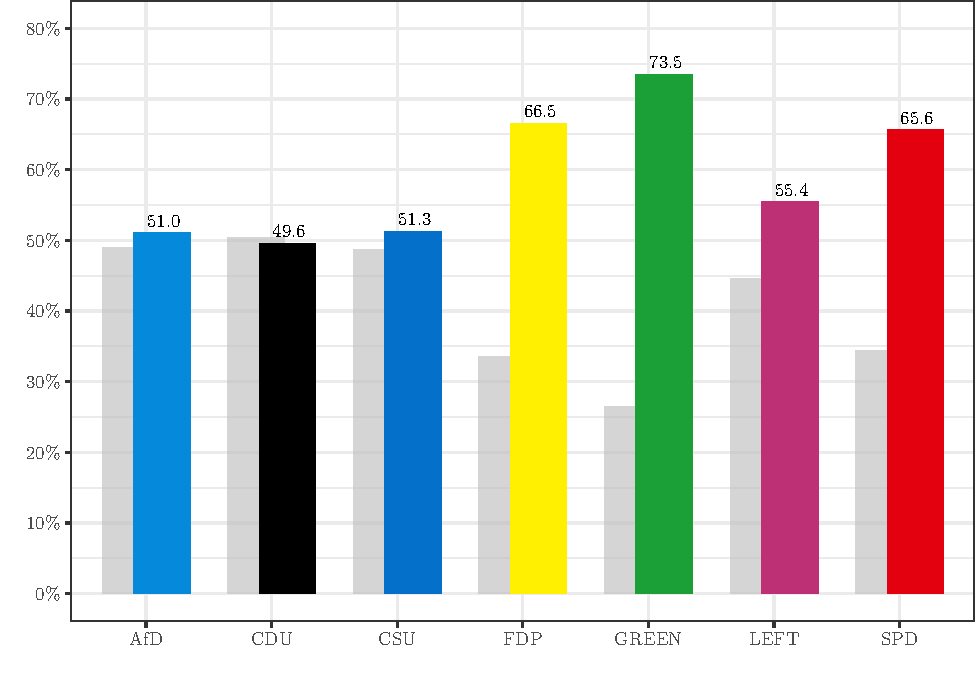
\includegraphics[width=0.95\linewidth]{thesis_files/figure-latex/plotpercentageaccount-1} \hfill{}

\caption{Percentage of Candidates with an Account on Twitter}\label{fig:plotpercentageaccount}
\end{figure}
\vspace{-1cm}
\begin{center}
    \begin{minipage}{0.95\linewidth}
    \scriptsize
    \textit{Note}: The colored bars represent the percentage of candidates with a Twitter account, while the grey bars indicate the percentage without one.
    \end{minipage}
\end{center}
\begin{figure}[H]

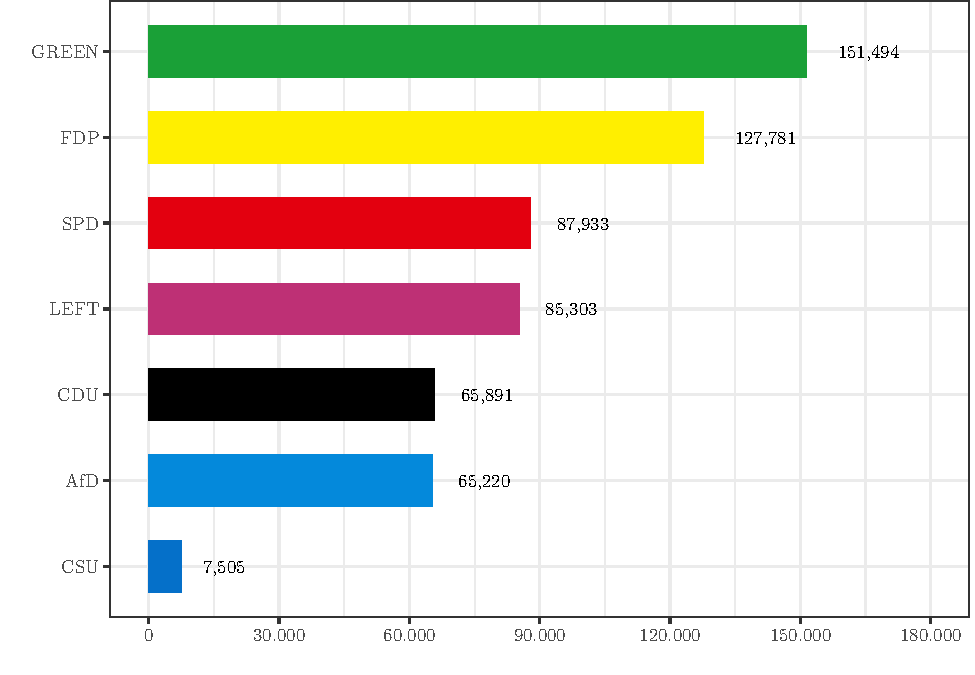
\includegraphics[width=0.95\linewidth]{thesis_files/figure-latex/plottweetsamountybyparty-1} \hfill{}

\caption{Number of Tweets posted by Party}\label{fig:plottweetsamountybyparty}
\end{figure}
\newpage

Figure \texttt{\ref{fig:tweetshist}} displays the distribution of tweets over the observation period. As one might expect, in the weeks leading up to the election, candidates are most active on Twitter, culminating in the day of the election. After the election, activity plummets shortly across all parties until, in December, the coalition negotiations for the new cabinet between the SPD, Greens, and FDP again boost the discourse on Twitter. However, the distribution for tweets over time is fairly consistent, thereby demonstrating that no individual events (at least not those that have no relevance to the content) influence the analysis.
\begin{figure}[H]

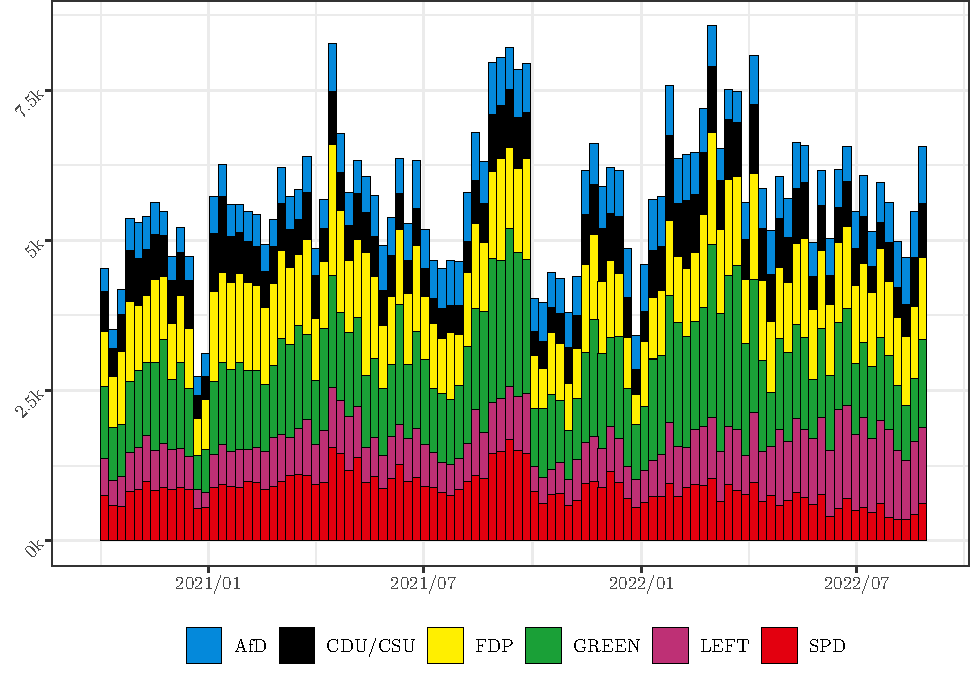
\includegraphics[width=0.95\linewidth]{thesis_files/figure-latex/tweetshist-1} \hfill{}

\caption{Party-wise Frequency of Tweets Over Time}\label{fig:tweetshist}
\end{figure}
\vspace{-1cm}
    \begin{minipage}{\linewidth}
    \begin{center}
    \scriptsize
    \textit{Note}: To improve readbility, CDU and CSU were grouped into one category.
    \end{center}
    \end{minipage}
In general, Figure \texttt{\ref{fig:plottweetsamountybyparty}} and \texttt{\ref{fig:tweetshist}} show that the volume of the text corpora definitely validate the feasibility of a quantitative sentiment analysis, for which the scores are calculated in the next steps.

\hypertarget{dv}{%
\subsubsection{Dependent Variable: Sentiment}\label{dv}}

To quantify the emotional tone expressed in each tweet, I employ the \emph{sentiment dictionary for German political language} developed by Christian Rauh (\protect\hyperlink{ref-rauhValidatingSentimentDictionary2018}{2018}). The dictionary is comprised of lists of terms categorized as either positive or negative and has been validated specifically for German political speech. In total, the dictionary contains 19,750 negative and 17,330 positive words as well as all corresponding negations. To use the dictionary, I cleaned the text data by removing unnecessary elements such as punctuation, account-handles and emojis with the \emph{quanteda} package (\protect\hyperlink{ref-benoitQuantedaPackageQuantitative2018}{Benoit et al. 2018}). Once cleaned, each tweet is analyzed for occurrences of positive and negative terms, drawn from the sentiment dictionary.
In the next step, the raw sentiment score is derived by subtracting the total number of occurrences of negative terms from the total number of occurrences of positive terms as noted in the following formula:

\textbf{Equation \eqref{eq:rawsentscore}}
\begin{equation}
\text{Raw Sentiment Score} = \sum (\text{Positive Terms}) - \sum (\text{Negative Terms})
\tag{1} 
\label{eq:rawsentscore}
\end{equation}
In order to control for varying tweet lengths, the raw sentiment score is standardized by dividing it by the total number of terms in each tweet.

\textbf{Equation \eqref{eq:standsentscore}}
\begin{equation}
\text{Standardized Sentiment Score} = \frac{\text{Raw Sentiment Score}}{\text{Total Number of Terms in Tweet}}
\tag{2} 
\label{eq:standsentscore}
\end{equation}
The output of this standardization process is the score that will serve as the dependent variable in the analysis and ranges between -1 and +1. A score of -1 reflects a highly negative sentiment, whereas +1 signifies a strongly positive sentiment. In the Appendix, Figure \texttt{\ref{fig:examplescoring}} provides a demonstration of the scoring process for a single tweet, Table \ref{tab:sumstats} depicts the summary statistics for the sentiment variables and Figure \texttt{\ref{fig:sentimenthist}} displays the distribution of the normalized sentiment score.\footnote{In section \protect\hyperlink{robustness}{\emph{5 Robustness Checks}}, the scoring process of the dictionary will be reflected in detail.}

\hypertarget{independent-variables}{%
\subsubsection{Independent Variables}\label{independent-variables}}

To test the hypotheses, I use multiple independent variables: (1) \emph{Incumbent} is a binary variable indicating if the account is representing a candidate of the current government parties, (2) \emph{Incumbent X Chancellor} is a binary variable indicating if the account is maintained by a candidate of the current chancellor's party, (3) \emph{Radical Right} is a binary variable indicating if the account is maintained by a candidate of the AfD, (4) \emph{Gender} is a binary variable indicating the candidate's gender, (5) \emph{Weeks to Election} indicates the time to the election in weeks, (6) \emph{Terms} indicates the total number of words in the tweet.

\hypertarget{methods}{%
\subsection{Methods}\label{methods}}

\hypertarget{model-specification}{%
\subsubsection{Model Specification}\label{model-specification}}

To discern how sentiment in key German political accounts is influenced, I employ a series of Ordinary Least Squares (OLS) regression models. The independent variables are added in a step wise manner across six different models, increasing in complexity from model 1 to model 6. The simplest model tests the effect of incumbency without any other controls is noted by the following formula:

\textbf{Equation \eqref{eq:regression}}
\begin{equation}
Y_{i} = \beta_{0} + \beta_{1} \cdot \text{Incumbent}_{i} + \epsilon_{i}
\tag{3} 
\label{eq:regression}
\end{equation}
where \(Y_{i}\) represents the normalized sentiment score, \(\beta_{0}\) is the intercept, \(\beta_{1}\) denotes the incumbency coefficient, and \(\epsilon_{i}\) is the error term. For all models this basic specification is the same, but based on the model \(\beta_{n}\) are added depending on the independent variables used. To investigate whether the presumed effects persist even over the change of governing parties I run two separate regressions: for all tweets posted before (\texttt{\ref{tab:regone}}) and after the election day (\texttt{\ref{tab:regtwo}}).

\hypertarget{results}{%
\section{Results}\label{results}}

First, I test the proposed hypotheses using OLS regressions and subsequently turn to examining the sentiment patterns over time. The regression results for all tweets before the 2021 election are provided in Table \ref{tab:regone}. Models 1 and 2 examine the link between positive sentiment and incumbency status. Models 3 and 4 include the party and candidate level variables, Models 5 and 6 the control variables.
\newpage
\begin{table}[H]
    \centering
    \caption{OLS Regression: Tweets one Year before the 2021 Election}
    \label{tab:regone}
\begingroup 
\scriptsize 
\begin{tabular}{@{\extracolsep{5pt}}lcccccc} 
\\[-1.8ex]\hline 
\hline \\[-1.8ex] 
 & \multicolumn{6}{c}{Dependent Variable: Normalized Sentiment Score} \\ 
\cline{2-7} 
\\[-1.8ex] & (1) & (2) & (3) & (4) & (5) & (6)\\ 
\hline \\[-1.8ex] 
 Incumbent & 0.019$^{***}$ & 0.015$^{***}$ & 0.010$^{***}$ & 0.011$^{***}$ & 0.011$^{***}$ & 0.008$^{***}$ \\ 
  & (0.001) & (0.001) & (0.001) & (0.001) & (0.001) & (0.001) \\ 
  & & & & & & \\ 
 Incumbent x Chancellor &  & 0.010$^{***}$ & 0.010$^{***}$ & 0.012$^{***}$ & 0.012$^{***}$ & 0.017$^{***}$ \\ 
  &  & (0.001) & (0.001) & (0.001) & (0.001) & (0.001) \\ 
  & & & & & & \\ 
 Radical Right &  &  & $-$0.035$^{***}$ & $-$0.031$^{***}$ & $-$0.031$^{***}$ & $-$0.031$^{***}$ \\ 
  &  &  & (0.001) & (0.001) & (0.001) & (0.001) \\ 
  & & & & & & \\ 
 Gender (Ref. Female) &  &  &  & 0.018$^{***}$ & 0.018$^{***}$ & 0.014$^{***}$ \\ 
  &  &  &  & (0.001) & (0.001) & (0.001) \\ 
  & & & & & & \\ 
 Weeks to Election &  &  &  &  & 0.0001$^{***}$ & 0.0002$^{***}$ \\ 
  &  &  &  &  & (0.00002) & (0.00002) \\ 
  & & & & & & \\ 
 Terms &  &  &  &  &  & $-$0.003$^{***}$ \\ 
  &  &  &  &  &  & (0.00003) \\ 
  & & & & & & \\ 
 Constant & 0.032$^{***}$ & 0.032$^{***}$ & 0.037$^{***}$ & 0.013$^{***}$ & 0.010$^{***}$ & 0.078$^{***}$ \\ 
  & (0.0004) & (0.0004) & (0.0004) & (0.001) & (0.001) & (0.001) \\ 
  & & & & & & \\ 
\hline \\[-1.8ex] 
Observations & 288,656 & 288,656 & 288,656 & 288,656 & 288,656 & 288,656 \\ 
R$^{2}$ & 0.002 & 0.003 & 0.006 & 0.008 & 0.008 & 0.053 \\ 
Adjusted R$^{2}$ & 0.002 & 0.003 & 0.006 & 0.008 & 0.008 & 0.053 \\ 
\hline 
\hline \\[-1.8ex] 
\end{tabular} 
\endgroup 
\vspace{0.5em} % Add some vertical space between the table and note
    \begin{minipage}{0.95\linewidth}
    \scriptsize
    \textit{Note}: Standard errors are in parentheses. Significance values are indicated with: $^*$p$<$0.1; $^{**}$p$<$0.05;
    $^{***}$p$<$0.01. The data includes all tweets posted by candidates prior to the 2021 German federal election (Timeframe:
    2020/09/26 - 2021/09/26). The Incumbent dummy equals 1 if the candidate is a member of the CDU/CDSU or SPD, 0 if otherwise. The
    Incumbent x Chancellor dummy equals 1 if the candidate is a member of the CDU/CSU, 0 if otherwise. The Radical Right dummy equals 1 if
    the candidate is a member of the AfD, 0 if otherwise. The Gender dummy equals 1 if the Candidate is male, 0 if female. 
    \end{minipage}
    \end{table}
\vspace{-.5cm}

The data suggests that being part of the incumbent party is associated with candidates utilizing a more positive sentiment during campaigns on Twitter. Model 1 indicates a \emph{0.019} increase on the normalized sentiment variable for the candidates of the CDU/CSU and SPD in contrast to those of the opposition parties. The size of this effect decreases with model complexity to \emph{0.008} in Model 6, however remains highly significant across all specifications. Accordingly, the data supports the main hypothesis \ref{hypothesis:H1} that incumbent parties employ a more positive sentiment in campaigns.
Model 2 introduces an additional layer of granularity with the inclusion of the \emph{Incumbent x Chancellor} dummy, showing a \emph{0.010} increase for the CDU/CSU candidates in contrast to all other parties including the SPD. Once controlling for all covariates, including tweet length and weeks until the election, the effect increases to \emph{0.017}. Accordingly, the model also provides evidence for \ref{hypothesis:H2} that it is mainly the CDU/CSU's candidates that drive the incumbency effect. Adding to this, Model 3 highlights a pronounced negative sentiment associated with radical right parties, consistent with the description of their campaign strategies and rhetoric. The dummy coefficient, presented in Model 3, for the \emph{Radical Right} (AfD) affiliated candidates points to a highly significant decrease of \emph{0.035} in the normalized sentiment variable. This means that, in comparison to all other parties, AfD candidates are more likely to employ a negative sentiment in their Twitter campaigns. Consequentially, the empirical findings support the idea outlined in \ref{hypothesis:H3}.
Shifting away from the party level effects, Model 4 includes the candidates' gender. This indicates a highly significant positive effect for male candidates with a coefficient of \emph{0.018}. Interestingly, the gender variable does not diminish the incumbency effect, implying that this is independent of a candidate's gender. This observation aligns with \ref{hypothesis:H4} which focuses on gender-based differences in emotive language. Confronted with the stereotype that women are too emotional, the results indicate that female candidates express less emotional language than their male counterparts.

Building upon the regression results, Figure \texttt{\ref{fig:plotintrapartydiversity}} shows the intra-party variance on the normalized sentiment variable. For this purpose, the account-level averages are calculated and their distribution within the parties plotted using kernel density estimation. Accordingly, the height of the curves represents the density of accounts with the corresponding average sentiment score. This allows to evaluate whether parties' candidates are uniform in terms of their emotive language strategies.
\newpage
\begin{figure}[H]

{\centering 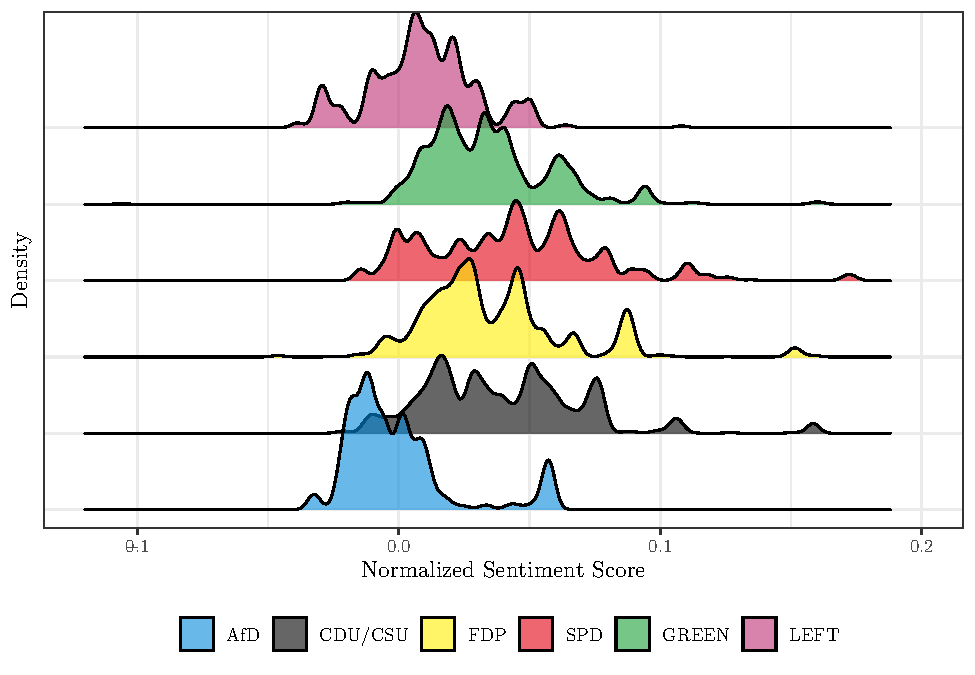
\includegraphics[width=1\linewidth]{thesis_files/figure-latex/plotintrapartydiversity-1} 

}

\caption{Intra-party Sentiment Diversity}\label{fig:plotintrapartydiversity}
\end{figure}
\vspace{-1cm}
    \begin{minipage}{\linewidth}
    \begin{center}
    \scriptsize
    \textit{Note}: The data distribution is calculated for each party using the Kernel Density Estimation (KDE).
    \end{center}
    \end{minipage}\vspace{0.2cm}
Interestingly, the emotional language of the candidates is quite heterogeneous for all parties. While this seems to vary from party to party, e.g., the representatives of the AfD are more similar in the emotional language they use on Twitter than the very diverse SPD, it appears that there are different factions within all parties that systematically use different emotional language. The data suggest that parties are not uniform actors in terms of their emotive strategies. It may indeed be a strategic decision, especially for the bigger, ideologically diverse parties, to appeal to different voters through differing emotive appeals. Correspondingly, this first glance supports \ref{hypothesis:H5}. However, this is just a first outlook; a thorough evaluation would require analyses that take intra-party factions, and candidates' mandate type into account, which is beyond the scope of this work.

Having outlined the sentiment employed before the election, the data also allows an evaluation of the parties' post-election emotive strategies, in this specific case even with a change of government. Accordingly, I plot the parties' normalized sentiment scores for the two years surrounding the election in Figure \texttt{\ref{fig:plotsentimentweekly}} and conduct the same regression analysis on tweets posted in the year after the election in Table \ref{tab:regtwo} to examine if the presented effects persist.

\newpage
\begin{figure}[H]

{\centering 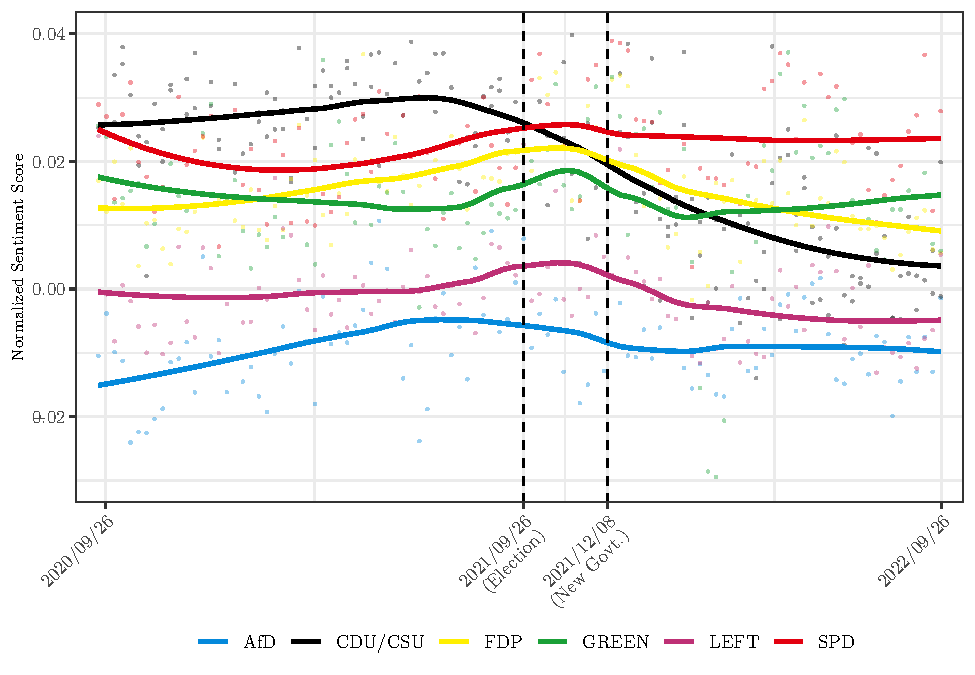
\includegraphics[width=0.95\linewidth]{thesis_files/figure-latex/plotsentimentweekly-1} 

}

\caption{Sentiment over Time}\label{fig:plotsentimentweekly}
\end{figure}
The emotive strategy of the CDU/CSU appears to have changed with the election. In line with the results in Table \ref{tab:regone}, in the preceding year, the candidates employed the most positive tone on Twitter with sentiment scores peaking at \emph{0.03} approximately three months before the election day. However, their use of positive sentiment began to steadily decrease immediately after, resulting in a new ranking of the parties along the sentiment score. In line with the theory, after being voted out of office, the CDU/CSU is clearly positioned as an opposition party that expresses more negative sentiment than the parties in government. Their former coalition partner, the SPD, which now leads the new government, demonstrates a contrasting trend: As the party remains in power, its candidates consistently tweet in a positive manner. However, the change from junior to a leading coalition partner does not appear to cause a significant incline in tone. The candidates of the SPD's coalition partners, the Greens \& FDP, exhibit a moderately positive sentiment that is fairly consistent over time, ranging from \emph{0.01} to \emph{0.02}. Notably, it does not seem to be an increase in their emotional tone, but rather the decrease in the CDU/CSU affiliated candidates that places them as the second and third most positive party after the election. Being voted out of office, particularly in this specific instance, seems to have a more pronounced effect on the candidates' tone than being voted into office. Those who previously held a mandate or at least believed they had a genuine shot at securing a seat, found themselves without one after the election. Possibly these particular candidates are driving the observed decline in the CDU/CSU's tone. As without a mandate, they might communicate their sentiments and opinions more directly and therefore possibly adopt a more negative language on Twitter.

Besides this, the SPD, FDP, Green and Left party all showed a brief upswing in positive language shortly before the election which peaks about a month before the formation of the new government. All of them, as potential coalition partners, played a role in regard to forming a new government. Therefore, it seems reasonable that in the weeks immediately before and after the election, the parties' candidates did not entirely focus on denouncing the status quo, but rather formulated their plans for the future. While doing so, they might have used a more positive sentiment, since they focused on their agenda and thus aimed to influence voters' perceptions in a positive way. Furthermore, the AfD and the Left, which were neither part of the first nor the later coalition, employ the most negative sentiment throughout the entire period. And unsurprisingly, as a radical right party, the AfD consistently displays the most negative language with none of the democratic parties employing a sentiment more negative than their candidates' at any time.

Finally, Table \ref{tab:regtwo} depicts the regression results for all tweets one year after the 2021 election. Exactly as in Table \ref{tab:regone}, Models 1 and 2 examine the link between sentiment and incumbency status. Models 3 and 4 include the party and candidate-level variables, Models 5 and 6 the control variables. In line with the change of government, the incumbent dummies are now recoded for the SPD-led coalition with the Greens and the FDP.

\newpage
\begin{table}[H]
    \centering
    \caption{OLS Regression: Tweets one Year after the 2021 Election}
    \label{tab:regtwo}
\begingroup 
\scriptsize 
\begin{tabular}{@{\extracolsep{5pt}}lcccccc} 
\\[-1.8ex]\hline 
\hline \\[-1.8ex] 
 & \multicolumn{6}{c}{Dependent Variable: Normalized Sentiment Score} \\ 
\cline{2-7} 
\\[-1.8ex] & (1) & (2) & (3) & (4) & (5) & (6)\\ 
\hline \\[-1.8ex] 
 Incumbent & 0.026$^{***}$ & 0.022$^{***}$ & 0.014$^{***}$ & 0.013$^{***}$ & 0.011$^{***}$ & 0.011$^{***}$ \\ 
  & (0.001) & (0.001) & (0.001) & (0.001) & (0.001) & (0.001) \\ 
  & & & & & & \\ 
 Incumbent x Chancellor.          &  & 0.021$^{***}$ & 0.021$^{***}$ & 0.023$^{***}$ & 0.021$^{***}$ & 0.018$^{***}$ \\ 
  &  & (0.001) & (0.001) & (0.001) & (0.001) & (0.001) \\ 
  & & & & & & \\ 
 Radical Right &  &  & $-$0.026$^{***}$ & $-$0.024$^{***}$ & $-$0.026$^{***}$ & $-$0.027$^{***}$ \\ 
  &  &  & (0.001) & (0.001) & (0.001) & (0.001) \\ 
  & & & & & & \\ 
 Gender (Ref. Female) &  &  &  & 0.015$^{***}$ & 0.014$^{***}$ & 0.015$^{***}$ \\ 
  &  &  &  & (0.001) & (0.001) & (0.001) \\ 
  & & & & & & \\ 
 Weeks to Election &  &  &  &  & 0.001$^{***}$ & 0.001$^{***}$ \\ 
  &  &  &  &  & (0.00002) & (0.00002) \\ 
  & & & & & & \\ 
 Terms &  &  &  &  &  & $-$0.003$^{***}$ \\ 
  &  &  &  &  &  & (0.00003) \\ 
  & & & & & & \\ 
 Constant & 0.016$^{***}$ & 0.016$^{***}$ & 0.024$^{***}$ & 0.004$^{***}$ & 0.028$^{***}$ & 0.080$^{***}$ \\ 
  & (0.001) & (0.001) & (0.001) & (0.001) & (0.001) & (0.001) \\ 
  & & & & & & \\ 
\hline \\[-1.8ex] 
Observations & 302,471 & 302,471 & 302,471 & 302,471 & 302,471 & 302,471 \\ 
R$^{2}$ & 0.005 & 0.007 & 0.008 & 0.010 & 0.014 & 0.047 \\ 
Adjusted R$^{2}$ & 0.005 & 0.007 & 0.008 & 0.010 & 0.014 & 0.047 \\ 
\hline 
\hline \\[-1.8ex] 
\end{tabular} 
\endgroup 
\vspace{0.5em} % Add some vertical space between the table and note
    \begin{minipage}{0.95\linewidth}
    \scriptsize
    \textit{Note}: Standard errors are in parentheses. Significance values are indicated with: $^*$p$<$0.1; $^{**}$p$<$0.05;
    $^{***}$p$<$0.01.
    The Data includes all tweets posted by candidates after the 2021 German federal election (Timeframe: 2021/09/26 - 2022/09/26).
    The Incumbent dummy equals 1 if the candidate is a member of the SPD, Grüne or FDP, 0 if otherwise. The Incumbent x Chancellor dummy
    equals 1 if the Candidate is a member of the SPD, 0 if otherwise. The Radical Right dummy equals 1 if the candidate is a
    member of the AfD, 0 if otherwise. The Gender dummy equals 1 if the candidate is male, 0 if female.
    \end{minipage}
    \end{table}\vspace{-.8cm}
Consistent with the party-level trends outlined in \texttt{\ref{fig:plotsentimentweekly}}, being part of the incumbent party is also associated with tweeting in a more positive manner in the new legislative period. Model 1 highlights this with a statistically significant coefficient of \emph{0.026}. Even as governments change, the positive tone of the incumbents' emotive language remains consistent. However, once controlling for all covariates, this effect decreases to \emph{0.011}. In this regard, it is noteworthy that, consistent with the findings in Table \ref{tab:regone}, accounting for all control variables, the \emph{Incumbent x Chancellor} coefficient is with a size of \emph{0.018} larger than the single \emph{Incumbent} effect. This suggests that now the SPD is the primary driver behind the positive tone in the new government and the Greens and FDP might not be as influenced by incumbency. This interpretation aligns well with the trends observed in Figure \texttt{\ref{fig:plotsentimentweekly}}. In general, it appears that the dynamics hypothesized in \ref{hypothesis:H1} and \ref{hypothesis:H2} are not limited to electioneering, but, although a bit weaker, permanently influence parties' communication on Twitter. Aside from this, the \emph{Gender} and \emph{Radical Right} coefficients are also consistent with those in Table \ref{tab:regone}, therefore as well seem robust to the change in government and point in time during the election cycle.

Finally, across all analyses presented, a pattern is apparent that sentiment scores seem to be centered closely around zero. Despite the trends and effects (mostly) aligning with the theory, the parties exhibit only minor variations in the second decimal place on the normalized sentiment variable. This might be attributed to the dictionary-based-method and computation of the dependent variable (see \protect\hyperlink{dv}{\emph{section 3.1.2}}). I will address this and, in general, provide a comprehensive assessment of the measurement and validity in the next section \protect\hyperlink{robustness}{\emph{5 Robustness Checks}}.

\hypertarget{robustness}{%
\section{Robustness Checks}\label{robustness}}

The small effect sizes in the analysis appear to stem from the distribution of the normalized sentiment scores (displayed in Figure \texttt{\ref{fig:sentimenthist}} in the Appendix). The majority of tweets receive a neutral score of zero with positive and negative scores around following the curve of a normal distribution. Therefore, despite the scores showing reasonable variance, when calculating party level averages they may balance each other out, which could be an explanation for the marginal differences in Figure \texttt{\ref{fig:plotsentimentweekly}} and effect sizes in Tables \ref{tab:regone} and \ref{tab:regtwo}. To address this, I rerun the main regression (Table \ref{tab:regone}) and trend analysis (Figure \texttt{\ref{fig:plotsentimentweekly}}) excluding all neutral coded Tweets with a score of 0. The results for this are depicted in Table \ref{tab:regoneneutral} and Figure \texttt{\ref{fig:plotsentimentweeklyappendix}} in the Appendix. The findings for the clearly positive or negative coded tweets correspond to the results of the main analysis, therefore suggesting it is not exclusively the tendency of the method to code tweets as neutral, which causes the small effects, but it is either due to a very balanced sentiment of the tweets or indicates that the dictionary does not capture sufficiently fine-grained sentiment differences in the text. Consequently, it is imperative to further validate the methodology and to verify whether the dictionary-based approach correctly measures the intended target dimension.

\hypertarget{validating-the-sentiment-dictionary}{%
\subsection{Validating the Sentiment Dictionary}\label{validating-the-sentiment-dictionary}}

\hypertarget{comparison-with-the-liwc-dictionary}{%
\subsubsection{Comparison with the LIWC Dictionary}\label{comparison-with-the-liwc-dictionary}}

In addition to the dictionary developed by Rauh (\protect\hyperlink{ref-rauhValidatingSentimentDictionary2018}{2018}), numerous other dictionaries find application in political science. To begin with, I want to test whether the results are robust to the choice of dictionary. For this I rerun the main regression (Table \ref{tab:regone}) with the LIWC's \emph{Tone} variable as dependent variable instead of the previously used normalized sentiment score. The LIWC software, as done in the analysis, reads the text word by word, compares each word with the glossary on which the program is based, and classifies the words. In this case, LIWC2015's German word lexicon was utilized. The \emph{Tone} variable ranges from 0 - 100 and is the result of the calculated difference between positive and negative words (\protect\hyperlink{ref-cohnLinguisticMarkersPsychological2004}{Cohn, Mehl, and Pennebaker 2004, 689}). Values of 50 indicate a neutral, higher values a more positive and lower values a more negative sentiment. The results for this regression are presented in Table \ref{tab:regliwcpreelection}.

I find that the results are robust to the choice of dictionary. Table \ref{tab:regliwcpreelection} with the \emph{LIWC-Tone} as dependent variable shows comparable effects to Table \ref{tab:regone}. Notably, all effects are larger with this approach. This, most likely, arises from the variable's scaling, which ranging from 0 - 100, offers a more intuitive interpretation compared to the normalized sentiment score with a span from -1 to 1. However, it might also be the case that the LIWC dictionary detects sentiment a bit differently. Nonetheless, in principle, the results confirm that the intended target dimension is correctly captured and, therefore, provide further support to the robustness of the findings.
\begin{table}[H]
    \centering
    \caption{OLS Regression: Tweets one Year before the 2021 Election (w/LIWC-Data)}
    \label{tab:regliwcpreelection}
\begingroup 
\scriptsize 
\begin{tabular}{@{\extracolsep{5pt}}lcccccc} 
\\[-1.8ex]\hline 
\hline \\[-1.8ex] 
 & \multicolumn{6}{c}{Dependent Variable: LIWC Tone} \\ 
\cline{2-7} 
\\[-1.8ex] & (1) & (2) & (3) & (4) & (5) & (6)\\ 
\hline \\[-1.8ex] 
 Incumbent & 5.452$^{***}$ & 3.709$^{***}$ & 2.775$^{***}$ & 2.887$^{***}$ & 2.887$^{***}$ & 3.034$^{***}$ \\ 
  & (0.171) & (0.208) & (0.211) & (0.211) & (0.212) & (0.211) \\ 
  & & & & & & \\ 
 Incumbent x Chancellor &  & 4.290$^{***}$ & 4.290$^{***}$ & 4.633$^{***}$ & 4.633$^{***}$ & 4.398$^{***}$ \\ 
  &  & (0.292) & (0.291) & (0.292) & (0.293) & (0.293) \\ 
  & & & & & & \\ 
 Radical Right &  &  & $-$6.365$^{***}$ & $-$5.937$^{***}$ & $-$5.937$^{***}$ & $-$5.938$^{***}$ \\ 
  &  &  & (0.263) & (0.265) & (0.265) & (0.265) \\ 
  & & & & & & \\ 
 Gender (Ref. Female) &  &  &  & 2.402$^{***}$ & 2.402$^{***}$ & 2.538$^{***}$ \\ 
  &  &  &  & (0.165) & (0.165) & (0.165) \\ 
  & & & & & & \\ 
 Weeks to Election &  &  &  &  & 0.0002 & $-$0.002 \\ 
  &  &  &  &  & (0.005) & (0.005) \\ 
  & & & & & & \\ 
 Terms &  &  &  &  &  & 0.130$^{***}$ \\ 
  &  &  &  &  &  & (0.006) \\ 
  & & & & & & \\ 
 Constant & 46.776$^{***}$ & 46.776$^{***}$ & 47.710$^{***}$ & 44.338$^{***}$ & 44.334$^{***}$ & 41.419$^{***}$ \\ 
  & (0.093) & (0.093) & (0.101) & (0.253) & (0.283) & (0.315) \\ 
  & & & & & & \\ 
\hline \\[-1.8ex] 
Observations & 288,320 & 288,320 & 288,320 & 288,320 & 288,320 & 288,320 \\ 
R$^{2}$ & 0.004 & 0.004 & 0.006 & 0.007 & 0.007 & 0.008 \\ 
Adjusted R$^{2}$ & 0.004 & 0.004 & 0.006 & 0.007 & 0.007 & 0.008 \\ 
\hline 
\hline \\[-1.8ex] 
\end{tabular} 
\endgroup 
\vspace{0.5em} % Add some vertical space between the table and note
    \begin{minipage}{0.95\linewidth}
    \scriptsize
    \textit{Note}: Standard errors are in parentheses. Significance values are indicated with: $^*$p$<$0.1; $^{**}$p$<$0.05;
    $^{***}$p$<$0.01. The Data includes all Tweets posted by candidates prior to the 2021 German federal election (Timeframe:
    2020/09/26 - 2021/09/26). The Incumbent dummy equals 1 if the candidate is a member of the CDU/CDSU or SPD, 0 if otherwise. The
    Incumbent x Chancellor dummy equals 1 if the candidate is a member of the CDU/CSU, 0 if otherwise. The Radical Right dummy equals 1 if
    the candidate is a member of the AfD, 0 if otherwise. The Gender dummy equals 1 if the candidate is male, 0 if female. 
    \end{minipage}
    \end{table}
\hypertarget{comparison-with-human-coded-sentiment}{%
\subsubsection{Comparison with Human Coded Sentiment}\label{comparison-with-human-coded-sentiment}}

While comparing scores with another dictionary provides some confidence in the sentiment measurement, it doesn't conclusively validate that dictionary-based methods can accurately detect a tweet's true tone. Tweets often contain elements of irony, wherein the expressed sentiment differs from the underlying intent, are context-dependent or include quotations. These intricate nuances might be overlooked when merely tallying the text's positive and negative words. Consequently, dictionary-based approaches may misinterpret a tweet's genuine tone, which, in reality, significantly influences the reader's perception. To address this, I cross-validated my results using human judgment. I randomly selected 200 tweets from the dataset and had them assessed by three coders (one of them being myself). Each coder read the tweets and coded the sentiment on a scale from -100 to 100.\footnote{Instead of the -1 to 1 scale I used this to provide the possibility of more fine grained judgment.} They were directed to rate the tweets independent of their own political beliefs and solely focus on the emotional language employed. Table \ref{tab:humancoders} offers a brief overview of the coders and Table \ref{tab:correlation} displays the Pearson correlations between the different coders and dictionary scores.
\begin{table}[H]
    \begin{center}
        \caption{Human Coders}
        \label{tab:humancoders}
        {\footnotesize
        \begin{tabularx}{\textwidth}{LCCC}
        \hline \hline
        & Coder 1 & Coder 2 & Coder 3 \\
        \hline
        Gender & male & female & female \\
        Age & 24 & 22 & 24\\
        \hline \hline
        \end{tabularx}}
    \end{center}
\end{table}
\begin{table}[H]
    \begin{center}
        \caption{Correlation Matrix for Coder and Dictionary Scores}
        \label{tab:correlation}
        {\footnotesize
        \begin{tabularx}{\textwidth}{LCCCCC}
        \hline \hline
                   & Coder 1 & Coder 2 & Coder 3 & Rauh Dic. & LIWC Dic. \\
        \hline
        Coder 1     & 1.0000 & 0.7939 & 0.7950 & 0.4040 & 0.4664 \\
        Coder 2     & 0.7939 & 1.0000 & 0.8677 & 0.4377 & 0.4928 \\
        Coder 3     & 0.7950 & 0.8677 & 1.0000 & 0.4538 & 0.5343 \\
        Rauh Dic.    & 0.4040 & 0.4377 & 0.4538 & 1.0000 & 0.4450 \\
        LIWC Dic.            & 0.4664 & 0.4928 & 0.5343 & 0.4450 & 1.0000 \\
        \hline \hline
        \end{tabularx}}
    \end{center}
\end{table}
\vspace{-.5cm}

The three coders appear to have a strong consensus regarding the sentiment of the tweets. Their scores indicate a high correlation, with Pearson's coefficients consistently exceeding \emph{0.7}. This suggest an important first finding: coders seem to be largely in agreement about a tweets emotive framing. However, the dictionary provided by Rauh (\protect\hyperlink{ref-rauhValidatingSentimentDictionary2018}{2018}), as well as by LIWC, are only moderately correlated with the hand coded scores. The Pearson correlations range from \emph{0.4 - 0.05}, indicating some, but not really compelling agreement. To further investigate this discrepancy between human and dictionary coding, I plot the values against each other in Figure \texttt{\ref{fig:humancoderscatter}}.
\begin{figure}[H]

{\centering 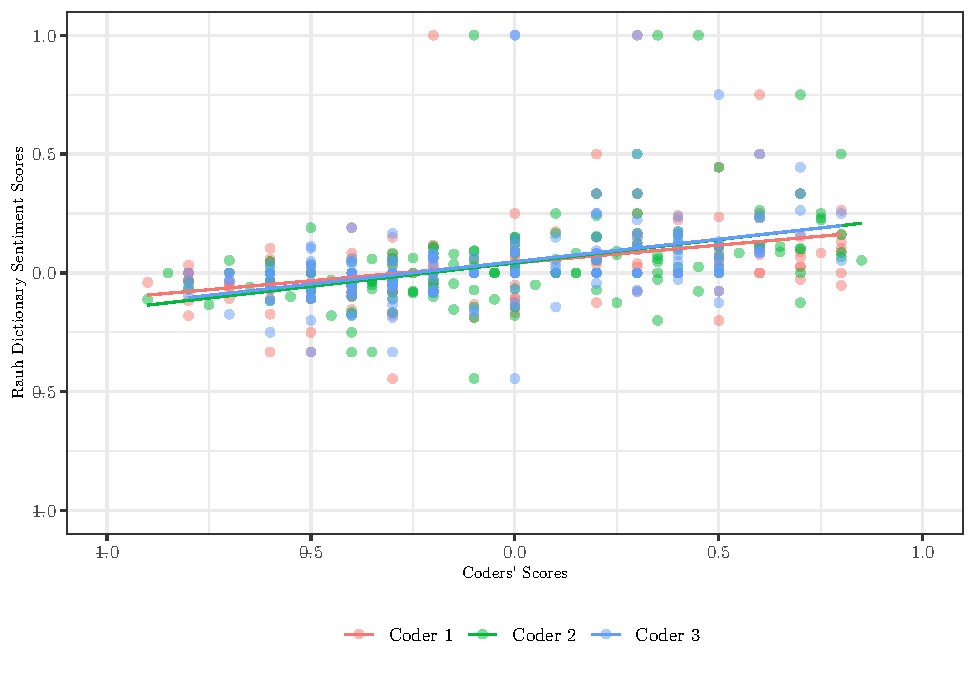
\includegraphics[width=1\linewidth]{thesis_files/figure-latex/humancoderscatter-1} 

}

\caption{Comparison between Coder and Dictionary Scores}\label{fig:humancoderscatter}
\end{figure}
The scatter plot visualizes the relationship between individual coders' and dictionary sentiment scores. Each point represents one tweet and coders are differentiated by color. For every coder, linear regression lines are drawn to highlight the variables association. The plot aligns with the correlation matrix and shows a moderate association of the scores. Especially noteworthy is that human coders tend to code tweets as far more emotional than the dictionary employed in this work. The coders identified a multitude of really negative tweets around the \emph{-0.9 - 0.7} range. For these, Rauh's sentiment dictionary only coded a slightly negative almost neutral score. Possibly the issues discussed, such as irony etc. influence this disagreement. Moreover, a couple tweets are coded as extremely positive by the dictionary, with the highest score possible of \emph{1}, which the coders identified as neutral or moderately positive. This most likely stems from short tweets with just one or two words. To exemplify this, I take a look at one of these tweets: On May 5, 2021 Katja Wilma Mast (SPD) posted: ``Empfehlung \url{https://t.co/Ip4dF26lVa}''

She references a URL link, which neither the coders nor the dictionary had access to. Since not being able to judge the content referenced, but noting the recommendation, coders indicated scores of \emph{0.3, 0.35} and \emph{0.3}. Contrary, Rauh's dictionary suggests a score of \emph{1}. This nicely illustrates the discussed shortcoming of the method being unable to understand context. Furthermore, even the normalized scores are still biased towards shorter texts, as one positive word on its own causes such a high score.

Given these considerations, the presented findings should be approached with caution and viewed more as preliminary indicators rather than definitive proof. It appears necessary to validate the results either through machine learning approaches or by further accounting for the context of tweets to ensure a more reliable measurement.

\hypertarget{time-frames}{%
\subsection{Time Frames}\label{time-frames}}

Aside from the dictionary measurement, I also want to account for specific time frames possibly driving the effects. To investigate this, I rerun the regression from Table \ref{tab:regone}, but limit the data to tweets posted within the three months leading up to the election. Similarly, I replicate the regression from Table \ref{tab:regtwo}, excluding tweets posted before the formation of the new government. The results of these analyses are detailed in Table \ref{tab:regcampaign} and \ref{tab:regnewgvt} in the Appendix. Both sets of findings align with the primary results, confirming that no specific time periods were responsible for the main effects discussed.

\hypertarget{conclusion}{%
\section{Conclusion}\label{conclusion}}

Voters critically assess the existing status quo and assess their contentment with the track record of the incumbent party when deciding whom to endorse. Aware of this evaluative mechanism, party representatives and candidates are incentivized to strategically influence voters' perceptions of the prevailing status quo in their favor. This is achieved not only through the substance and emphasis of their campaigns but also through the use of emotional appeals.

Understanding candidates' emotional strategies, especially in the realm of social media, is pivotal in today's digital age. Therefore, in this study, I expand the findings provided by Crabtree et al. (\protect\hyperlink{ref-crabtreeItNotOnly2020}{2020}) on strategic emotions in electioneering by studying the sentiment of parliamentary candidates around the 20th German federal election. I find that incumbency, especially for candidates affiliated with the chancellor's party, is associated with a more positive sentiment on Twitter. Furthermore, the results indicate substantial intra-party diversity, with candidates of the same party utilizing quite differing sentiments on Twitter. Lastly, I observe significant variation between female and male candidates on Twitter. The results suggest that female candidates, possibly in response to societal stereotypes, tweet in a more neutral emotional tone than their male counterparts.

However, all results presented should be taken with great caution. The cross-validation conducted with three coders suggests that dictionary-based methods do not capture sentiment in the same manner as human interpretation. I find that the dictionaries provided by Rauh (\protect\hyperlink{ref-rauhValidatingSentimentDictionary2018}{2018}) and LIWC (\protect\hyperlink{ref-meierLIWCAufDeutsch2019}{Meier et al. 2019}) neither correlate sufficiently with hand-coded sentiment scores. As a consequence, this study provides a valuable starting point concerning the examination of candidates' emotional strategies. However, future research should employ more nuanced measurements, such as machine learning approaches, or sentiment dictionaries with a more fine-grained coding of tweet context or references. Aside from the measurement issues, subsequent research could delve into comparative analyses, explore mechanisms on other campaigning platforms, or examine the outlined intra-party diversity in more detail.

\hypertarget{references}{%
\section*{References}\label{references}}
\addcontentsline{toc}{section}{References}

\noindent

\setlength{\parindent}{-0.5cm}
\setlength{\leftskip}{0.5cm}
\setlength{\parskip}{8pt}

\hypertarget{refs}{}
\begin{CSLReferences}{1}{0}
\leavevmode\vadjust pre{\hypertarget{ref-adamsAnybodyListeningEvidence2011}{}}%
Adams, James, Lawrence Ezrow, and Zeynep Somer-Topcu. 2011. {``\href{https://doi.org/10.1111/j.1540-5907.2010.00489.x}{Is {Anybody Listening}? {Evidence That Voters Do Not Respond} to {European Parties}' {Policy Statements During Elections}}.''} \emph{American journal of political science} 55(2): 370--82.

\leavevmode\vadjust pre{\hypertarget{ref-barrieAcademictwitteRPackageAccess2021}{}}%
Barrie, Christopher, and Justin Ho. 2021. {``\href{https://doi.org/10.21105/joss.03272}{{academictwitteR}: An {R} Package to Access the {Twitter Academic Research Product Track} V2 {API} Endpoint}.''} \emph{Journal of Open Source Software} 6(62): 3272.

\leavevmode\vadjust pre{\hypertarget{ref-benoitQuantedaPackageQuantitative2018}{}}%
Benoit, Kenneth et al. 2018. {``\href{https://doi.org/10.21105/joss.00774}{Quanteda: {An R} Package for the Quantitative Analysis of Textual Data}.''} \emph{Journal of Open Source Software} 3(30): 774.

\leavevmode\vadjust pre{\hypertarget{ref-boussalisGenderCandidateEmotional2021}{}}%
Boussalis, Constantine, Travis G. Coan, Mirya R. Holman, and Stefan Müller. 2021. {``\href{https://doi.org/10.1017/S0003055421000666}{Gender, {Candidate Emotional Expression}, and {Voter Reactions During Televised Debates}}.''} \emph{American Political Science Review} 115(4): 1242--57.

\leavevmode\vadjust pre{\hypertarget{ref-braderCampaigningHeartsMinds2006}{}}%
Brader, Ted. 2006. \emph{Campaigning for Hearts and Minds: {How} Emotional Appeals in Political Ads Work}. {Chicago and London}: {The University of Chicago Press}.

\leavevmode\vadjust pre{\hypertarget{ref-castanhosilvaPoliticiansUnleashedPolitical2022}{}}%
Castanho Silva, Bruno, and Sven-Oliver Proksch. 2022. {``\href{https://doi.org/10.1017/psrm.2021.36}{Politicians Unleashed? {Political} Communication on {Twitter} and in Parliament in {Western Europe}}.''} \emph{Political Science Research and Methods} 10(4): 776--92.

\leavevmode\vadjust pre{\hypertarget{ref-choCampaignTonePolitical2013}{}}%
Cho, Jaeho. 2013. {``\href{https://doi.org/10.1111/jcom.12064}{Campaign {Tone}, {Political Affect}, and {Communicative Engagement}}.''} \emph{Journal of communication} 63(6): 1130--52.

\leavevmode\vadjust pre{\hypertarget{ref-cohnLinguisticMarkersPsychological2004}{}}%
Cohn, Michael A, Matthias R Mehl, and James W Pennebaker. 2004. {``\href{https://doi.org/10.1111/j.0956-7976.2004.00741.x}{Linguistic {Markers} of {Psychological Change Surrounding September} 11, 2001}.''} \emph{Psychological science} 15(10): 687--93.

\leavevmode\vadjust pre{\hypertarget{ref-crabtreeItNotOnly2020}{}}%
Crabtree, Charles, Matt Golder, Thomas Gschwend, and H. Indriason Indrii. 2020. {``\href{https://doi.org/10.1086/707613}{It {Is Not Only What You Say}, {It Is Also How You Say It}: {The Strategic Use} of {Campaign Sentiment}}.''} \emph{The Journal of politics} 82(3): 1044--60.

\leavevmode\vadjust pre{\hypertarget{ref-debusParteienwettbewerbUndWahrscheinlichkeit2022}{}}%
Debus, Marc. 2022. {``\href{https://doi.org/10.1007/s11615-021-00361-8}{Parteienwettbewerb Und {Wahrscheinlichkeit} Verschiedener {Koalitionsoptionen} Bei Der {Bundestagswahl} 2021}.''} \emph{Politische Vierteljahresschrift} 63(1): 73--88.

\leavevmode\vadjust pre{\hypertarget{ref-debusEconomicVotingCoalition2014}{}}%
Debus, Marc, Mary Stegmaier, and Jale Tosun. 2014. {``\href{https://doi.org/10.1017/psrm.2013.16}{Economic {Voting} Under {Coalition Governments}: {Evidence} from {Germany}}.''} \emph{Political Science Research and Methods} 2(1): 49--67.

\leavevmode\vadjust pre{\hypertarget{ref-deckerWahljahr20212021}{}}%
Decker, Frank. 2021. {``{Das Wahljahr 2021}.''} \emph{bpb.de}.

\leavevmode\vadjust pre{\hypertarget{ref-duchVoterPerceptionsAgenda2013}{}}%
Duch, Raymond, and Randolph Stevenson. 2013. {``\href{https://doi.org/10.1016/j.electstud.2013.05.013}{Voter Perceptions of Agenda Power and Attribution of~Responsibility for Economic Performance}.''} \emph{Economics and Elections: Effects Deep and Wide} 32(3): 512--16.

\leavevmode\vadjust pre{\hypertarget{ref-durikEthnicityGenderStereotypes2006}{}}%
Durik, Amanda M. et al. 2006. {``\href{https://doi.org/10.1007/s11199-006-9020-4}{Ethnicity and {Gender Stereotypes} of {Emotion}}.''} \emph{Sex Roles} 54(7): 429--45.

\leavevmode\vadjust pre{\hypertarget{ref-falterHandbuchWahlforschung2014}{}}%
Falter, Jürgen W., and Harald Schoen, eds. 2014. \emph{Handbuch {Wahlforschung}}. 2nd ed. {Wiesbaden}: {Springer VS}.

\leavevmode\vadjust pre{\hypertarget{ref-fennisPsychologyAdvertising2016}{}}%
Fennis, Bob Michaël, and Wolfgang Stroebe. 2016. \emph{The Psychology of Advertising}. 2nd ed. {London ; New York}: {Routledge Taylor \& Francis Group}.

\leavevmode\vadjust pre{\hypertarget{ref-frascaWordsWeaponsLabeling2022}{}}%
Frasca, Teresa J., Emily A. Leskinen, and Leah R. Warner. 2022. {``\href{https://doi.org/10.1177/03616843221123745}{Words {Like Weapons}: {Labeling Women As Emotional During} a {Disagreement Negatively Affects} the {Perceived Legitimacy} of {Their Arguments}}.''} \emph{Psychology of Women Quarterly} 46(4): 420--37.

\leavevmode\vadjust pre{\hypertarget{ref-freedmanCampaignAdvertisingDemocratic2004}{}}%
Freedman, Paul, Michael Franz, and Kenneth Goldstein. 2004. {``\href{https://doi.org/10.1111/j.0092-5853.2004.00098.x}{Campaign {Advertising} and {Democratic Citizenship}}.''} \emph{American Journal of Political Science} 48(4): 723--41.

\leavevmode\vadjust pre{\hypertarget{ref-gleasonMerePresenceGender2020}{}}%
Gleason, Shane A. 2020. {``\href{https://doi.org/10.1177/1065912919847001}{Beyond {Mere Presence}: {Gender Norms} in {Oral Arguments} at the {U}.{S}. {Supreme Court}}.''} \emph{Political Research Quarterly} 73(3): 596--608.

\leavevmode\vadjust pre{\hypertarget{ref-greeneLeadershipCompetitionDisagreement2016}{}}%
Greene, Zachary, and Matthias Haber. 2016. {``\href{https://doi.org/10.1017/S0007123414000283}{Leadership {Competition} and {Disagreement} at {Party National Congresses}}.''} \emph{British Journal of Political Science} 46(3): 611--32.

\leavevmode\vadjust pre{\hypertarget{ref-grossGamePracticalGuide2016}{}}%
Gross, Lina et al. 2016. {``Game {On}! {A} Practical Guide to {Campaigning}.''}

\leavevmode\vadjust pre{\hypertarget{ref-hargraveDoubleStandardGender2023}{}}%
Hargrave, Lotte. 2023. {``\href{https://doi.org/10.1017/S0007123422000515}{A {Double Standard}? {Gender Bias} in {Voters}' {Perceptions} of {Political Arguments}}.''} \emph{British Journal of Political Science} 53(2): 327--45.

\leavevmode\vadjust pre{\hypertarget{ref-jungherrTwitterUseElection2016}{}}%
Jungherr, Andreas. 2016. {``\href{https://doi.org/10.1080/19331681.2015.1132401}{Twitter Use in Election Campaigns: {A} Systematic Literature Review}.''} \emph{Journal of Information Technology \& Politics} 13(1): 72--91.

\leavevmode\vadjust pre{\hypertarget{ref-kercherWahlprogrammeAlsPflichtubung2013}{}}%
Kercher, Jan, and Frank Brettschneider. 2013. {``\href{https://doi.org/10.1007/978-3-658-01328-8_12}{Wahlprogramme Als {Pflichtübung}? {Typen}, {Funktionen} Und {Verständlichkeit} Der {Bundestagswahlprogramme} 1994\textendash 2009}.''} : 269--90.

\leavevmode\vadjust pre{\hypertarget{ref-keyResponsibleElectorateRationality1966}{}}%
Key, Valdimer Orlando, and Milton C. Cummings. 1966. \emph{The {Responsible Electorate}: {Rationality} in {Presidential Voting} 1936-1960}. {Cambridge, Mass}: {Harvard University Press}.

\leavevmode\vadjust pre{\hypertarget{ref-konigEPINetzTwitterPoliticians2022}{}}%
König, Tim. 2022. {``\href{https://doi.org/10.7802/2415}{{EPINetz Twitter Politicians} 2021}.''} \emph{Politische Vierteljahresschrift}.

\leavevmode\vadjust pre{\hypertarget{ref-lehmannManifestoProjectDataset2023}{}}%
Lehmann, Pola et al. 2023. {``\href{https://doi.org/10.25522/MANIFESTO.MPDS.2023A}{Manifesto {Project Dataset}}.''}

\leavevmode\vadjust pre{\hypertarget{ref-marcusAffectiveIntelligencePolitical2000}{}}%
Marcus, George E. 2000. \emph{Affective Intelligence and Political Judgment}. eds. W. Russell Neuman and Michael MacKuen. {Chicago}: {University of Chicago Press}.

\leavevmode\vadjust pre{\hypertarget{ref-marcusAnxietyEnthusiasmVote1993}{}}%
Marcus, George E., and Michael B. MacKuen. 1993. {``\href{https://doi.org/10.2307/2938743}{Anxiety, {Enthusiasm}, and the {Vote}: {The Emotional Underpinnings} of {Learning} and {Involvement During Presidential Campaigns}}.''} \emph{American Political Science Review} 87(3): 672--85.

\leavevmode\vadjust pre{\hypertarget{ref-mayerTwoDimensionsNarcissistic2020}{}}%
Mayer, Sabrina J., Carl C. Berning, and David Johann. 2020. {``\href{https://doi.org/10.1002/per.2228}{The {Two Dimensions} of {Narcissistic Personality} and {Support} for the {Radical Right}: {The Role} of {Right}\textendash{{Wing Authoritarianism}}, {Social Dominance Orientation} and {Anti}\textendash{{Immigrant Sentiment}}}.''} \emph{European Journal of Personality} 34(1): 60--76.

\leavevmode\vadjust pre{\hypertarget{ref-meierLIWCAufDeutsch2019}{}}%
Meier, Tabea et al. 2019. \emph{\href{https://doi.org/10.31234/osf.io/uq8zt}{"{LIWC} Auf {Deutsch}": {The Development}, {Psychometrics}, and {Introduction} of {DE-LIWC2015}}}.

\leavevmode\vadjust pre{\hypertarget{ref-muddePopulistRadicalRight2007}{}}%
Mudde, Cas. 2007. \emph{\href{https://doi.org/10.1017/CBO9780511492037}{Populist {Radical Right Parties} in {Europe}}}. {Cambridge}: {Cambridge University Press}.

\leavevmode\vadjust pre{\hypertarget{ref-muellerTwitterMadeMe2022}{}}%
Mueller, Samuel David, and Marius Saeltzer. 2022. {``\href{https://doi.org/10.1080/1369118X.2020.1850841}{Twitter Made Me Do It! {Twitter}'s Tonal Platform Incentive and Its Effect on Online Campaigning}.''} \emph{Information, Communication \& Society} 25(9): 1247--72.

\leavevmode\vadjust pre{\hypertarget{ref-naiGoingNegativeWorldwide2020}{}}%
Nai, Alessandro. 2020. {``\href{https://doi.org/10.1017/gov.2018.32}{Going {Negative}, {Worldwide}: {Towards} a {General Understanding} of {Determinants} and {Targets} of {Negative Campaigning}}.''} \emph{Government and Opposition} 55(3): 430--55.

\leavevmode\vadjust pre{\hypertarget{ref-naiFearLoathingPopulist2021}{}}%
---------. 2021. {``\href{https://doi.org/10.1080/15377857.2018.1491439}{Fear and {Loathing} in {Populist Campaigns}? {Comparing} the {Communication Style} of {Populists} and {Non-populists} in {Elections Worldwide}}.''} \emph{Journal of Political Marketing} 20(2): 219--50.

\leavevmode\vadjust pre{\hypertarget{ref-neubergerInternetJournalismusVomTraditionellen2010}{}}%
Neuberger, Christoph, and Thorsten Quandt. 2010. {``\href{https://doi.org/10.1007/978-3-531-92437-3_3}{Internet-{Journalismus}: {Vom} Traditionellen {Gatekeeping} Zum Partizipativen {Journalismus}?}''}

\leavevmode\vadjust pre{\hypertarget{ref-plesciaRetrospectiveVotingParty2017}{}}%
Plescia, Carolina, and Sylvia Kritzinger. 2017. {``\href{https://doi.org/10.1080/17457289.2016.1243543}{Retrospective Voting and Party Support at Elections: Credit and Blame for Government and Opposition}.''} \emph{Journal of Elections, Public Opinion and Parties} 27(2): 156--71.

\leavevmode\vadjust pre{\hypertarget{ref-rauhValidatingSentimentDictionary2018}{}}%
Rauh, Christian. 2018. {``\href{https://doi.org/10.1080/19331681.2018.1485608}{Validating a Sentiment Dictionary for {German} Political Language\textemdash a Workbench Note}.''} \emph{Journal of Information Technology \& Politics} 15(4): 319--43.

\leavevmode\vadjust pre{\hypertarget{ref-ridoutItMyCampaign2011}{}}%
Ridout, Travis N., and Kathleen Searles. 2011. {``\href{https://doi.org/10.1111/j.1467-9221.2010.00819.x}{It's {My Campaign I}'ll {Cry} If {I Want} to: {How} and {When Campaigns Use Emotional Appeals}}.''} \emph{Political Psychology} 32(3): 439--58.

\leavevmode\vadjust pre{\hypertarget{ref-saltzerTwitterAccountsCandidates2021}{}}%
Sältzer, Marius et al. 2021. {``\href{https://doi.org/10.4232/1.13790}{Twitter Accounts of Candidates in the {German} Federal Election 2021 ({GLES})}.''}

\leavevmode\vadjust pre{\hypertarget{ref-saltzerFindingBirdWings2022}{}}%
Sältzer, Marius. 2022. {``\href{https://doi.org/10.1177/1354068820957960}{Finding the Bird's Wings: {Dimensions} of Factional Conflict on {Twitter}}.''} \emph{Party Politics} 28(1): 61--70.

\leavevmode\vadjust pre{\hypertarget{ref-saeltzerBundestagswahl2021Auf2022}{}}%
Sältzer, Marius, and Sebastian Stier. 2022. {``\href{https://doi.org/10.15464/EASY.2022.05}{{Die Bundestagswahl 2021 auf Twitter}}.''} \emph{easy\_social\_sciences} (67): 30--38.

\leavevmode\vadjust pre{\hypertarget{ref-schmidtWoerterbuchZurPolitik2010}{}}%
Schmidt, Manfred G. 2010. \emph{{Wörterbuch zur Politik}}. 3rd ed. {Stuttgart}: {Kröner}.

\leavevmode\vadjust pre{\hypertarget{ref-schoenWahlkampfforschung2014}{}}%
Schoen, Harald. 2014. {``\href{https://doi.org/10.1007/978-3-658-05164-8_16}{Wahlkampfforschung}.''} In \emph{Handbuch {Wahlforschung}}, eds. Jürgen W. Falter and Harald Schoen. {Wiesbaden}: {Springer Fachmedien Wiesbaden}, 661--728.

\leavevmode\vadjust pre{\hypertarget{ref-stierElectionCampaigningSocial2018}{}}%
Stier, Sebastian, Arnim Bleier, Haiko Lietz, and Markus Strohmaier. 2018. {``\href{https://doi.org/10.1080/10584609.2017.1334728}{Election {Campaigning} on {Social Media}: {Politicians}, {Audiences}, and the {Mediation} of {Political Communication} on {Facebook} and {Twitter}}.''} \emph{Political Communication} 35(1): 50--74.

\leavevmode\vadjust pre{\hypertarget{ref-utychNegativeAffectiveLanguage2018}{}}%
Utych, Stephen M. 2018. {``\href{https://doi.org/10.1177/1532673X17693830}{Negative {Affective Language} in {Politics}}.''} \emph{American Politics Research} 46(1): 77--102.

\leavevmode\vadjust pre{\hypertarget{ref-valentinoElectionNightAlright2011}{}}%
Valentino, Nicholas A. et al. 2011. {``\href{https://doi.org/10.1017/S0022381610000939}{Election {Night}'s {Alright} for {Fighting}: {The Role} of {Emotions} in {Political Participation}}.''} \emph{The Journal of Politics} 73(1): 156--70.

\leavevmode\vadjust pre{\hypertarget{ref-valentinoWorriedCitizenGood2008}{}}%
Valentino, Nicholas A., Vincent L. Hutchings, Antoine J. Banks, and Anne K. Davis. 2008. {``Is a {Worried Citizen} a {Good Citizen}? {Emotions}, {Political Information Seeking}, and {Learning} via the {Internet}.''} \emph{Political Psychology} 29(2): 247--73. \url{https://www.jstor.org/stable/20447114} (June 21, 2022).

\leavevmode\vadjust pre{\hypertarget{ref-vavreckMessageMattersEconomy2009}{}}%
Vavreck, Lynn. 2009. \emph{The Message Matters: The Economy and Presidential Campaigns}. {Princeton, N.J}: {Princeton University Press}.

\leavevmode\vadjust pre{\hypertarget{ref-vogelsPartisanDifferencesSocial2021}{}}%
Vogels, Emily A., Brooke Auxier, and Monica Anderson. 2021. \emph{Partisan Differences in Social Media Use Show up for Some Platforms, but Not {Facebook}}. {Pew Research Center}.

\leavevmode\vadjust pre{\hypertarget{ref-weberEmotionsCampaignsPolitical2013}{}}%
Weber, Christopher. 2013. {``\href{https://doi.org/10.1177/1065912912449697}{Emotions, {Campaigns}, and {Political Participation}}.''} \emph{Political Research Quarterly} 66(2): 414--28.

\leavevmode\vadjust pre{\hypertarget{ref-widmannHowEmotionalAre2021}{}}%
Widmann, Tobias. 2021. {``\href{https://doi.org/10.1111/pops.12693}{How {Emotional Are Populists Really}? {Factors Explaining Emotional Appeals} in the {Communication} of {Political Parties}}.''} \emph{Political Psychology} 42(1): 163--81.

\end{CSLReferences}
\indent
\setlength{\parindent}{17pt}
\setlength{\leftskip}{0pt}
\setlength{\parskip}{0pt}

\newpage
\appendix

\hypertarget{appendix}{%
\section{Appendix}\label{appendix}}

\hypertarget{figures}{%
\subsection{Figures}\label{figures}}
\begin{figure}[H]

{\centering 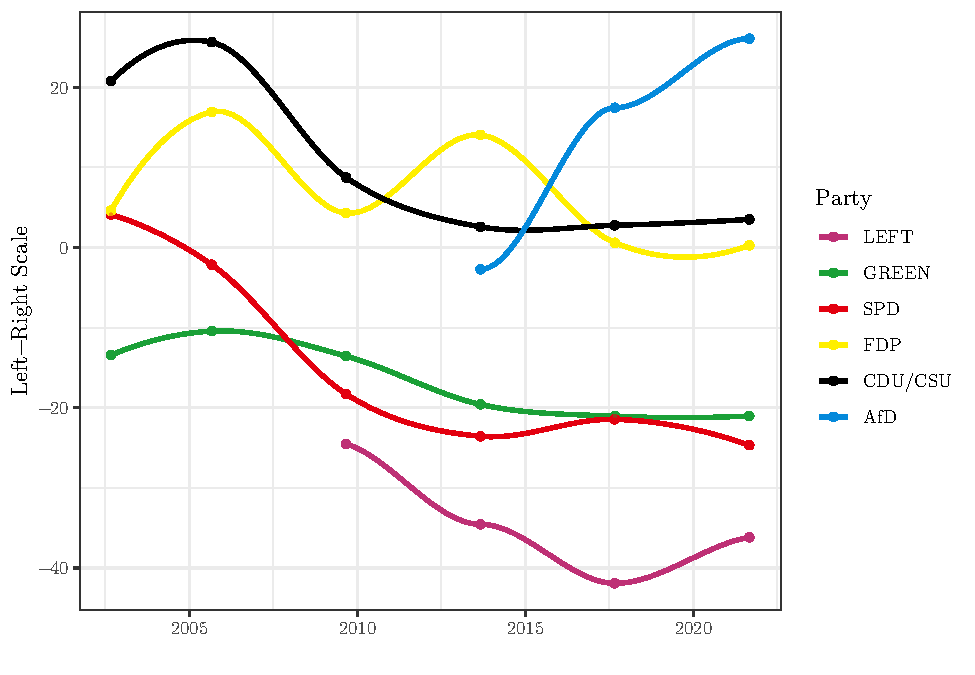
\includegraphics[width=1\linewidth]{thesis_files/figure-latex/partypositions-1} 

}

\caption{German Parties' Positions}\label{fig:partypositions}
\end{figure}
\vspace{-0.3cm}
\begin{center}
    \begin{minipage}{\linewidth}
    \scriptsize
    \textit{Note}: The data is from the Manifesto Data Collection (Version 2023a). The left-right scale represents the party's
    position, as measured by the RILE score. A negative score indicates a more left ideology and a positive score a more right ideology.
    \end{minipage}
\end{center}
\newpage
\begin{figure}[H]

{\centering \includegraphics[width=1\linewidth]{../../02_data/03_tables_figures/example_scoring} 

}

\caption{Demonstration of the Sentiment Scoring}\label{fig:examplescoring}
\end{figure}
\newpage
\begin{figure}[H]

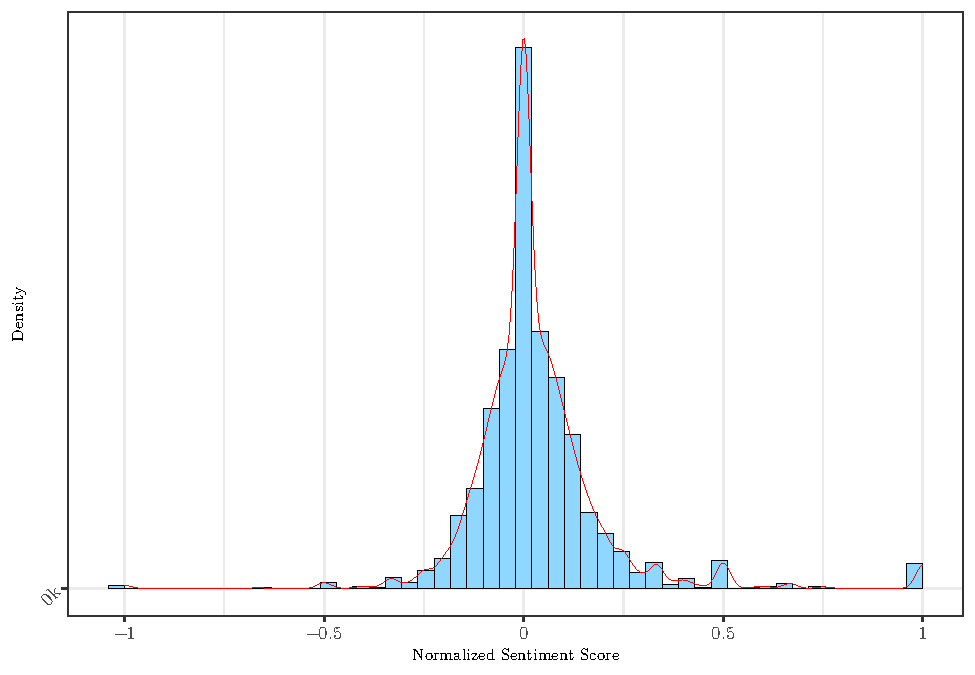
\includegraphics[width=0.95\linewidth]{thesis_files/figure-latex/sentimenthist-1} \hfill{}

\caption{Distribution of Normalized Sentiment Scores}\label{fig:sentimenthist}
\end{figure}
\newpage
\begin{figure}[H]

{\centering 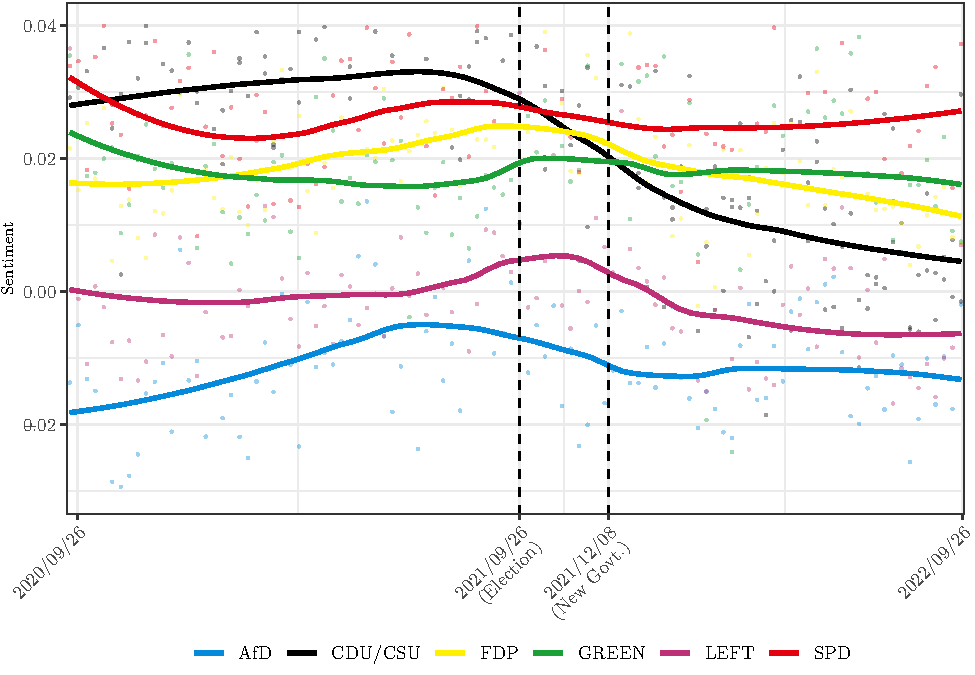
\includegraphics[width=1\linewidth]{thesis_files/figure-latex/plotsentimentweeklyappendix-1} 

}

\caption{Sentiment over Time (w/o neutral tweets)}\label{fig:plotsentimentweeklyappendix}
\end{figure}
\vspace{-0.2cm}
\begin{center}
    \begin{minipage}{\linewidth}
    \scriptsize
    \textit{Note}: All Tweets with a normalized sentiment score of zero are excluded.
    Every point indicates a week's average sentiment of candidates from one party.
    The data points have been smoothed using a locally weighted scatterplot smoothing (LOESS) approach. In this plot,
    a span of 0.6 was chosen to balance the trade-off between capturing the local structure and maintaining a global perspective on
    sentiment trends. 
    \end{minipage}
\end{center}
\hypertarget{tables}{%
\subsection{Tables}\label{tables}}
\begin{table}[H]
    \begin{center}
        \caption{Variables included in the Tweets-Dataset}
        \label{tab:apptable}
        {\footnotesize
        \begin{tabularx}{\textwidth}{LCC} % Adjust the column types
        \hline \hline
        Variable Name & Type & Source \\
        \hline
        tweet\_id & Categorical & Twitter API \\
        twitter\_handle & Categorical & Twitter API \\
        text & Text Data & Twitter API \\
        text\_clean & Text Data & Twitter API \\
        tweet\_date & Categorical & Twitter API \\
        retweet\_count & Date & Twitter API \\
        like\_count & Continuous & Twitter API \\
        quote\_count & Continuous & Twitter API \\
        name & Continuous & Twitter API \\
        gender & Categorical & GLES / EPIN \\
        party & Categorical & GLES / EPIN \\
        district\_name & Categorical & GLES / EPIN \\
        district\_number & Categorical & GLES / EPIN \\
        region & Categorical & GLES / EPIN \\
        incumbent & Categorical & GLES / EPIN \\
        listed\_candidate & Binary & GLES \\
        direct\_candidate & Binary & GLES \\
        binary\_federal\_parliamentarian & Binary & GLES \\
        binary\_state\_parliamentarian & Binary & EPIN \\
        binary\_european\_parliamentarian & Binary & EPIN \\
        binary\_federal\_state\_secretary & Binary & EPIN \\
        binary\_state\_state\_secretary & Binary & EPIN \\
        binary\_federal\_minister & Binary & EPIN \\
        binary\_state\_minister & Binary & EPIN \\
        user\_verified & Binary & EPIN \\
        user\_location & Binary & Twitter API \\
        user\_created\_at & Categorical & Twitter API \\
        user\_url & Date & Twitter API \\
        user\_tweet\_count & Categorical & Twitter API \\
        user\_list\_count & Continuous & Twitter API \\
        user\_followers\_count & Continuous & Twitter API \\
        user\_following\_count & Continuous & Twitter API \\
        terms & Continuous & Twitter API \\
        \hline \hline
        \end{tabularx}}
    \end{center}
\end{table}
\newpage
\begin{table}[!htb]
    \centering
    \caption{Summary Statistics: Sentiment Variables}
    \label{tab:sumstats}
\begin{tabular}{@{\extracolsep{5pt}}lccccc} 
\\[-1.8ex]\hline 
\hline \\[-1.8ex] 
Statistic & \multicolumn{1}{c}{N} & \multicolumn{1}{c}{Mean} & \multicolumn{1}{c}{St. Dev.} & \multicolumn{1}{c}{Min} & \multicolumn{1}{c}{Max} \\ 
\hline \\[-1.8ex] 
Positive Terms & 591,127 & 1.66 & 1.63 & 0 & 35 \\ 
Negative Terms & 591,127 & 1.37 & 1.54 & 0 & 16 \\ 
Raw Sentiment Score & 591,127 & 0.29 & 2.10 & $-$16 & 35 \\ 
Standardized Sentiment Score & 591,127 & 0.03 & 0.18 & $-$1.00 & 1.00 \\ 
\hline \\[-1.8ex] 
\end{tabular} 
\end{table}
\newpage
\begin{table}[H]
    \centering
    \caption{OLS Regression: Tweets one Year before the 2021 Election (w/o neutral Tweets)}
    \label{tab:regoneneutral}
\begingroup 
\scriptsize 
\begin{tabular}{@{\extracolsep{5pt}}lcccccc} 
\\[-1.8ex]\hline 
\hline \\[-1.8ex] 
 & \multicolumn{6}{c}{Dependent Variable: Normalized Sentiment Score} \\ 
\cline{2-7} 
\\[-1.8ex] & (1) & (2) & (3) & (4) & (5) & (6)\\ 
\hline \\[-1.8ex] 
 Incumbent & 0.025$^{***}$ & 0.021$^{***}$ & 0.014$^{***}$ & 0.016$^{***}$ & 0.016$^{***}$ & 0.011$^{***}$ \\ 
  & (0.001) & (0.001) & (0.001) & (0.001) & (0.001) & (0.001) \\ 
  & & & & & & \\ 
 Incumbent x Chancellor &  & 0.009$^{***}$ & 0.009$^{***}$ & 0.013$^{***}$ & 0.012$^{***}$ & 0.020$^{***}$ \\ 
  &  & (0.002) & (0.002) & (0.002) & (0.002) & (0.002) \\ 
  & & & & & & \\ 
 Radical Right &  &  & $-$0.046$^{***}$ & $-$0.042$^{***}$ & $-$0.042$^{***}$ & $-$0.042$^{***}$ \\ 
  &  &  & (0.002) & (0.002) & (0.002) & (0.001) \\ 
  & & & & & & \\ 
 Gender (Ref. Female) &  &  &  & 0.024$^{***}$ & 0.024$^{***}$ & 0.018$^{***}$ \\ 
  &  &  &  & (0.001) & (0.001) & (0.001) \\ 
  & & & & & & \\ 
 Weeks to Election &  &  &  &  & 0.0001$^{***}$ & 0.0002$^{***}$ \\ 
  &  &  &  &  & (0.00003) & (0.00003) \\ 
  & & & & & & \\ 
 Terms &  &  &  &  &  & $-$0.005$^{***}$ \\ 
  &  &  &  &  &  & (0.00003) \\ 
  & & & & & & \\ 
 Constant & 0.043$^{***}$ & 0.043$^{***}$ & 0.050$^{***}$ & 0.017$^{***}$ & 0.014$^{***}$ & 0.132$^{***}$ \\ 
  & (0.001) & (0.001) & (0.001) & (0.001) & (0.002) & (0.002) \\ 
  & & & & & & \\ 
\hline \\[-1.8ex] 
Observations & 214,996 & 214,996 & 214,996 & 214,996 & 214,996 & 214,996 \\ 
R$^{2}$ & 0.003 & 0.003 & 0.008 & 0.011 & 0.011 & 0.092 \\ 
Adjusted R$^{2}$ & 0.003 & 0.003 & 0.008 & 0.011 & 0.011 & 0.092 \\ 
\hline 
\hline \\[-1.8ex] 
\end{tabular} 
\endgroup 
\vspace{0.5em} % Add some vertical space between the table and note
    \begin{minipage}{0.95\linewidth}
    \scriptsize
    \textit{Note}: Standard errors are in parentheses. Significance values are indicated with: $^*$p$<$0.1; $^{**}$p$<$0.05;
    $^{***}$p$<$0.01. The data includes Tweets posted by candidates prior to the 2021 German federal election (Timeframe:
    2020/09/26 - 2021/09/26). In this case, all Tweets with a neutral normalized sentiment score of zero were excluded. The Incumbent dummy equals 1 if the candidate is a member of the CDU/CDSU or SPD, 0 if otherwise. The
    Incumbent x Chancellor dummy equals 1 if the candidate is a member of the CDU/CSU, 0 if otherwise. The Radical Right dummy equals 1 if
    the candidate is a member of the AfD, 0 if otherwise. The Gender dummy equals 1 if the candidate is male, 0 if female. 
    \end{minipage}
    \end{table}
\newpage
\begin{table}[H]
    \centering
    \caption{OLS Regression: Tweets three months before the 2021 Election}
    \label{tab:regcampaign}
\begingroup 
\scriptsize 
\begin{tabular}{@{\extracolsep{5pt}}lcccccc} 
\\[-1.8ex]\hline 
\hline \\[-1.8ex] 
 & \multicolumn{6}{c}{Dependent Variable: Normalized Sentiment Score} \\ 
\cline{2-7} 
\\[-1.8ex] & (1) & (2) & (3) & (4) & (5) & (6)\\ 
\hline \\[-1.8ex] 
 Incumbent & 0.021$^{***}$ & 0.017$^{***}$ & 0.013$^{***}$ & 0.013$^{***}$ & 0.013$^{***}$ & 0.008$^{***}$ \\ 
  & (0.001) & (0.002) & (0.002) & (0.002) & (0.002) & (0.002) \\ 
  & & & & & & \\ 
 Incumbent x Chancellor &  & 0.011$^{***}$ & 0.011$^{***}$ & 0.012$^{***}$ & 0.012$^{***}$ & 0.020$^{***}$ \\ 
  &  & (0.002) & (0.002) & (0.002) & (0.002) & (0.002) \\ 
  & & & & & & \\ 
 Radical Right &  &  & $-$0.024$^{***}$ & $-$0.023$^{***}$ & $-$0.022$^{***}$ & $-$0.023$^{***}$ \\ 
  &  &  & (0.002) & (0.002) & (0.002) & (0.002) \\ 
  & & & & & & \\ 
 Gender (Ref. Female) &  &  &  & 0.013$^{***}$ & 0.013$^{***}$ & 0.012$^{***}$ \\ 
  &  &  &  & (0.001) & (0.001) & (0.001) \\ 
  & & & & & & \\ 
 Weeks to Election &  &  &  &  & $-$0.0001 & 0.0001 \\ 
  &  &  &  &  & (0.0002) & (0.0002) \\ 
  & & & & & & \\ 
 Terms &  &  &  &  &  & $-$0.002$^{***}$ \\ 
  &  &  &  &  &  & (0.00005) \\ 
  & & & & & & \\ 
 Constant & 0.024$^{***}$ & 0.024$^{***}$ & 0.028$^{***}$ & 0.010$^{***}$ & 0.011$^{***}$ & 0.053$^{***}$ \\ 
  & (0.001) & (0.001) & (0.001) & (0.002) & (0.002) & (0.002) \\ 
  & & & & & & \\ 
\hline \\[-1.8ex] 
Observations & 80,948 & 80,948 & 80,948 & 80,948 & 80,948 & 80,948 \\ 
R$^{2}$ & 0.003 & 0.003 & 0.006 & 0.007 & 0.007 & 0.030 \\ 
Adjusted R$^{2}$ & 0.003 & 0.003 & 0.006 & 0.007 & 0.007 & 0.029 \\ 
\hline 
\hline \\[-1.8ex] 
\end{tabular} 
\endgroup 
\vspace{0.5em} % Add some vertical space between the table and note
    \begin{minipage}{0.95\linewidth}
    \scriptsize
    \textit{Note}: Standard errors are in parentheses. Significance values are indicated with: $^*$p$<$0.1; $^{**}$p$<$0.05;
    $^{***}$p$<$0.01.
    The data includes all Tweets posted by candidates three months prior to the 2021 German federal election (Timeframe: 2021/06/26 -
    2021/09/26).
    The Incumbent dummy equals 1 if the candidate is a member of the CDU/CDSU or SPD, 0 if otherwise. The Incumbent x Chancellor Dummy
    equals 1 if the candidate is a member of the CDU/CSU, 0 if otherwise. The Radical Right dummy equals 1 if the candidate is a
    member of the AfD, 0 if otherwise. The Gender dummy equals 1 if the candidate is male, 0 if female. 
    \end{minipage}
    \end{table}\clearpage
\begin{table}[H]
    \centering
    \caption{OLS Regression: Tweets after the new Government was formed}
    \label{tab:regnewgvt}
\begingroup 
\scriptsize 
\begin{tabular}{@{\extracolsep{5pt}}lcccccc} 
\\[-1.8ex]\hline 
\hline \\[-1.8ex] 
 & \multicolumn{6}{c}{Dependent Variable: Normalized Sentiment Score} \\ 
\cline{2-7} 
\\[-1.8ex] & (1) & (2) & (3) & (4) & (5) & (6)\\ 
\hline \\[-1.8ex] 
 Incumbent & 0.025$^{***}$ & 0.021$^{***}$ & 0.015$^{***}$ & 0.014$^{***}$ & 0.013$^{***}$ & 0.013$^{***}$ \\ 
  & (0.001) & (0.001) & (0.001) & (0.001) & (0.001) & (0.001) \\ 
  & & & & & & \\ 
 Incumbent x Chancellor &  & 0.021$^{***}$ & 0.021$^{***}$ & 0.022$^{***}$ & 0.022$^{***}$ & 0.019$^{***}$ \\ 
  &  & (0.001) & (0.001) & (0.001) & (0.001) & (0.001) \\ 
  & & & & & & \\ 
 Radical Right &  &  & $-$0.020$^{***}$ & $-$0.018$^{***}$ & $-$0.019$^{***}$ & $-$0.020$^{***}$ \\ 
  &  &  & (0.001) & (0.001) & (0.001) & (0.001) \\ 
  & & & & & & \\ 
 Gender (Ref. Female) &  &  &  & 0.015$^{***}$ & 0.015$^{***}$ & 0.015$^{***}$ \\ 
  &  &  &  & (0.001) & (0.001) & (0.001) \\ 
  & & & & & & \\ 
 Weeks to Election &  &  &  &  & 0.001$^{***}$ & 0.0005$^{***}$ \\ 
  &  &  &  &  & (0.00003) & (0.00003) \\ 
  & & & & & & \\ 
 Terms &  &  &  &  &  & $-$0.002$^{***}$ \\ 
  &  &  &  &  &  & (0.00003) \\ 
  & & & & & & \\ 
 Constant & 0.012$^{***}$ & 0.012$^{***}$ & 0.018$^{***}$ & $-$0.002$^{*}$ & 0.016$^{***}$ & 0.066$^{***}$ \\ 
  & (0.001) & (0.001) & (0.001) & (0.001) & (0.002) & (0.002) \\ 
  & & & & & & \\ 
\hline \\[-1.8ex] 
Observations & 250,188 & 250,188 & 250,188 & 250,188 & 250,188 & 250,188 \\ 
R$^{2}$ & 0.005 & 0.006 & 0.007 & 0.009 & 0.010 & 0.041 \\ 
Adjusted R$^{2}$ & 0.005 & 0.006 & 0.007 & 0.009 & 0.010 & 0.041 \\ 
\hline 
\hline \\[-1.8ex] 
\end{tabular} 
\endgroup 
\vspace{0.5em} % Add some vertical space between the table and note
    \begin{minipage}{0.95\linewidth}
    \scriptsize
    \textit{Note}: Standard errors are in parentheses. Significance values are indicated with: $^*$p$<$0.1; $^{**}$p$<$0.05;
    $^{***}$p$<$0.01.
    The data includes all Tweets posted by candidates after the formation of the new government (Timeframe: 2021/12/08 - 2022/09/26).
    The Incumbent dummy equals 1 if the Candidate is a member of the SPD, Grüne or FDP, 0 if otherwise. The Incumbent x Chancellor
    equals 1 if the candidate is a member of the SPD, 0 if otherwise. The Radical Right dummy equals 1 if the candidate is a
    member of the AfD, 0 if otherwise. The Gender dummy equals 1 if the candidate is male, 0 if female.
    \end{minipage}
    \end{table}\clearpage
% change rmd_files in `_bookdown.yml` files to determine order
% note that references and appendix are also contained here.

% --------------------------------------------
% --- last page: Declaration of Authorship ---
% --------------------------------------------

\newpage
\thispagestyle{empty}
\hypertarget{declaration-of-authorship}{%
\section*{Declaration of Authorship}\label{declaration-of-authorship}}
\textit{English}
\vspace{0.2cm}
\\
\noindent
I hereby declare that my thesis is the result of my own work and that I have marked all sources, including online sources, which have been cited without changes or in modified form, especially sources of texts, graphics, tables and pictures. I assure that I have not submitted this thesis for any other examination yet.
\vspace{0.5cm}
\\
\noindent
I am aware that in case of any breach of these rules procedure concering fraud or attempted fraud wil be taken in accordance with the subject-specific examinition regulations and/or the Allgemeine Satzung für Studien- und Prüfungsangelegenheiten (ASSP) or the Allgemeine Satzung zur Regelung von Zulassung, Studium und Prüfung der Humboldt-Universität zu Berlin (ZSP-HU).
\vspace{0.5cm}
\\
\noindent
\textit{German}
\vspace{0.2cm}
\\
\noindent
\noindent Hiermit erkläre ich, dass ich die vorliegende Abschlussarbeit selbständing verfasst habe und sämtliche Quellen, einschließlich Internetquellen, die unverändert oder abgewandelt wiedergegeben werden, insbesondere Quellen für Texte, Grafiken, Tabellen und Bilder, als solche kenntliche gemacht habe.
\vspace{0.5cm}
\\
\noindent
Ich versichere, dass ich die vorliegende Abschlussarbeit noch nicht für andere Prüfungen eingereicht habe. Mir ist bekannt, dass bei Verstößen gegen diese Grundsätze ein Verfahren wegen Täuschungsversuch bzw. Täuschung gemäß der fachspezifischen Prüfungsordnung und/oder der Allgemeinen Satzung für Studien- und Prüfungsangelegenheiten (ASSP) bzw. der Fachübergreifenden Satzung zur Regelung von Zulassung, Studium und Prüfung der Humboldt-Universität zu Berlin (ZSP-HU) eingeleitet wird.

\vspace{1cm}
\noindent
Berlin, \thesisdate{}
\vspace{3cm}
\\
\noindent
. . . . . . . . . . . . . . . . . . . . . . . . . . . . . . .
\vspace{0.1cm}

\thesisauthor{}


\end{document}
